% !TeX encoding = UTF-8

\documentclass[binding=0.6cm, english]{sapthesis}

\usepackage{microtype}
\usepackage[utf8]{inputenc}
\usepackage{hyperref}
\usepackage{graphicx}
\usepackage{booktabs}
\usepackage{listings}
\usepackage{xcolor}
\usepackage{amsmath}
\usepackage{url}
\usepackage{tikz}
\usetikzlibrary{positioning, arrows.meta, shapes.geometric, shapes.symbols,
                fit, calc, backgrounds, decorations.pathreplacing}

% --- Float placement tuning ---
\usepackage[section]{placeins}
\renewcommand{\topfraction}{0.9}      % up to 90% of a page may be top floats
\renewcommand{\bottomfraction}{0.8}
\renewcommand{\textfraction}{0.07}    % require only 7% text on a mixed page
\renewcommand{\floatpagefraction}{0.75}
\setcounter{topnumber}{3}
\setcounter{bottomnumber}{2}
\setcounter{totalnumber}{4}

% --- Thesis metadata ---
\title{Edits, Deletions, and Restrictions: Making Telegram's Content Dynamics Observable at Scale}
\author{Gabriel Alonso Bustamante}
\IDnumber{1983278}
\course{Applied Computer Science and Artificial Intelligence}
\courseorganizer{Dipartimento di Informatica}
\AcademicYear{2025/2026}
\advisor{Prof. Alessandro Mei}
\authoremail{bustamante.1983278@studenti.uniroma1.it}
\copyyear{2026}
\coadvisor{Dr. Alberto M. Mongardini}
\thesistype{Internship report}
\examdate{23 July 2026}
\examiner{Prof. Casalicchio}
\examiner{Prof. Cenciarelli}
\examiner{Prof. Masi}
\examiner{Prof. Mei}

% --- Hyperref setup ---
\hypersetup{
    colorlinks=true,
    linkcolor=black,
    citecolor=black,
    urlcolor=blue,
}

% --- Code listing style ---
\lstset{
    basicstyle=\ttfamily\small,
    breaklines=true,
    frame=single,
    numbers=left,
    numberstyle=\tiny,
    keywordstyle=\color{blue},
    commentstyle=\color{gray},
    stringstyle=\color{red},
}

\begin{document}

\frontmatter

% Suppress word-splitting (hyphenation) on the title page
\begingroup
\hyphenpenalty=10000
\exhyphenpenalty=10000
\maketitle
\endgroup

% \dedication{To ...}  % uncomment to add a dedication

\begin{abstract}

Public Telegram research corpora are snapshots: they record each channel once and miss the edits, deletions, and metadata changes that follow. This thesis presents TGDataset2, built by a single-worker scraper that repeatedly revisits public channels, recurses into their discussion groups, and on each visit detects edits and deletions and snapshots channel metadata, all within Telegram's rate limits on one machine.

The corpus trades breadth for depth: $12{,}065$ channels revisited over time and $475$ million messages, adding the edit (with before-and-after text), deletion, and longitudinal-metadata layers that no prior general-purpose corpus collected, together with a structured engagement-and-comment surface. These layers correct readings taken from the raw flags (the raw edit flag alone over-counts genuine editing roughly tenfold) and drive a method-led showcase on the 2026 US/Israel--Iran war.

\end{abstract}

\begin{acknowledgments}

I wish to thank my parents, for their support, given without conditions.

To my siblings goes my gratitude, for giving me the foundations of who I am today.

A heartfelt thanks to my friends, who stood by me through every exam, every deadline, and every doubt.

I am grateful to my professors, for giving life and character to equations and definitions.

I thank my psychotherapist, whose contribution to the conclusion of this journey may or may not be a spurious correlation.

Finally, I thank my co-advisor, for his infinite patience and for seeing this work through to the end with me.

\end{acknowledgments}


\tableofcontents

\mainmatter

\chapter{Introduction}
\label{chap:introduction}

Telegram is one of the central venues for public, large-scale, and often consequential communication: news distribution, political mobilisation, crisis information, and harmful content, whose presence on the platform is by now well documented in the research literature~\cite{baumgartner2020,walther2021,hoseini2024,propaganda2025}. As of early 2026 the platform reports more than a billion monthly active users, and its public \emph{channels}, one-to-many broadcast feeds with optional linked discussion groups, are where much of this public activity happens. Unlike the closed graphs of most social platforms, Telegram exposes channels and their content through a documented client API, which makes systematic collection possible. This has produced a small number of valuable research corpora, but they share a structural limitation: they are snapshots. Even the corpora that reach beyond broadcast channels into discussion groups and user accounts record each object as it existed at collection time, and discard almost everything that makes a channel a living object over time.

Prior corpora store a single \texttt{edit\_date} timestamp but not the before-and-after text of edits, so what an edit changed is unknowable. They do not track deletions, so moderation is invisible. They keep one metadata reading per channel, so they cannot say how a channel's title, picture, subscriber count, or restriction flags evolved. Several do not recurse into the linked groups where audiences reply either, leaving the comment layer absent, and even the corpora that do collect it captured each thread only once, frozen at collection time. The result is that a large class of questions, about content volatility, moderation, platform restriction, and audience interaction over time, cannot be answered from the existing public record, however large that record is.

This thesis addresses that gap with a system and a dataset built for longitudinal tracking and per-channel richness rather than channel count. The system is a single-worker scraper that visits public channels repeatedly, recurses into their discussion groups, and on each visit detects edits and deletions and snapshots channel metadata. The resulting corpus, TGDataset2, is deliberately a smaller set of channels, each revisited over time, and it adds the temporal layers, message edits, deletions, and metadata evolution, that no prior general-purpose Telegram corpus collected. The remainder of the thesis substantiates this claim and then exercises the new layers on real analyses.

\section*{Contributions}

This thesis makes the following contributions:

\begin{enumerate}
  \item \textbf{A scraper system} for deep, longitudinal collection of public Telegram channels, including recursive discussion-group collection, per-visit edit and deletion detection, and an alignment protocol for temporally consistent snapshots, all engineered to run continuously within the platform's rate limits on a single machine (Chapter~\ref{chap:methodology}).

  \item \textbf{The TGDataset2 corpus}: a deliberately smaller set of channels, each revisited over time, so it captures how content and channels change rather than a single snapshot (Section~\ref{sec:res-corpus}), and from which we reconstruct the forward graph and correct several common misreadings of it (Section~\ref{sec:res-network}).

  \item \textbf{A current-events showcase} that exercises several of the new layers at once on the 2026 US/Israel--Iran war response, leading with method (per-cohort indexing, pooled-vs-median decomposition, an exogenous timing clock) rather than raw volume (Section~\ref{sec:res-war}).
\end{enumerate}

\section*{Thesis outline}

Chapter~\ref{chap:background} surveys the Telegram platform and the existing public datasets, positioning this work against them. Chapter~\ref{chap:methodology} describes the scraper system: its architecture, the snowball channel-discovery mechanism, the database schema, the combined scraping pass that performs message collection together with edit and deletion detection, the alignment snapshot protocol, and the robustness features that allow reliable continuous operation. Chapter~\ref{chap:results} turns the corpus into evidence, characterising what it is, reconstructing the forward graph and correcting common misreadings of it, presenting the new capability layers together with the per-platform restriction-reason signal, and exercising them on the war showcase. Chapter~\ref{chap:conclusion} consolidates the limitations, restates the outcomes, and outlines future work.

\chapter{Background and Related Work}
\label{chap:background}

This chapter provides the context for our work. We begin with an overview of Telegram as a platform, then outline the research phenomena that make it a consequential subject of study, and finally survey prior efforts to build Telegram datasets.

%----------------------------------------------------------------------
\section{Telegram as a Platform}
\label{sec:telegram-platform}
%----------------------------------------------------------------------

Telegram is a cloud-based instant messaging application founded in 2013 by brothers Nikolai and Pavel Durov~\cite{telegram2026}.
Originally conceived as a privacy-oriented alternative to mainstream messaging services, the platform has grown rapidly: it surpassed 400~million monthly active users (MAU) in April~2020, reached 900~million MAU by March~2024, and crossed the one-billion-MAU threshold in March~2025~\cite{telegramstats2025}.
This trajectory makes Telegram one of the most widely used communication platforms in the world, trailing only WhatsApp (3~billion MAU~\cite{whatsapp2025}) and WeChat (1.41~billion MAU~\cite{wechat2025}).

Telegram's architecture distinguishes between several communication primitives~\cite{telegramfaq}.
\emph{Private chats} (one-to-one) and \emph{group chats} (up to 200\,000 members) support bidirectional messaging~\cite{telegramfaq}.
\emph{Channels}, by contrast, are broadcast-only spaces where a small set of administrators publish posts that are delivered to an unlimited number of subscribers~\cite{telegramchannels}.
Channels are the primary unit of analysis in our work: they function as one-to-many broadcasting media, much like public social-media feeds, while remaining indexed by a stable numeric identifier and an optional public username.
A channel can additionally be associated with a \emph{linked discussion group}, which turns each broadcast post into a comment thread~\cite{telegramdiscussion}.

%----------------------------------------------------------------------
\section{Why Telegram Warrants Study}
\label{sec:why-telegram}
%----------------------------------------------------------------------

Telegram's research importance follows first from its sheer reach.
Since crossing the one-billion-MAU threshold in March~2025~\cite{telegramstats2025}, Telegram has joined the small set of platforms that reach a meaningful fraction of the world's Internet users.
Despite this reach, it remains markedly under-studied relative to X~(formerly Twitter), Reddit, or Facebook~\cite{propaganda2025}.
The asymmetry between the platform's cultural and political weight and its empirical coverage motivates sustained corpus-building and observational work on Telegram.

Beyond scale, Telegram has become a venue for phenomena that matter to political, social, and security research.
It has carried communication around major elections, most recently the 2024~U.S.\ Presidential race~\cite{blas2025}, and functioned as a primary information channel during the Russo-Ukrainian war for both state-aligned media and wartime narratives~\cite{hanley2024,kloo2024}.
In authoritarian contexts it has hosted protest coordination and drawn targeted bans, notably in Iran and Russia~\cite{akbari2019}, and its performance and perception as a political actor in such settings has itself drawn scholarly scrutiny~\cite{wijermars2022}.
The platform has also absorbed communities displaced from mainstream networks: studies of extreme Internet celebrities and far-right actors document a migration to Telegram coincident with enforcement waves elsewhere~\cite{rogers2020,urman2022}, and subsequent work has characterised the resulting far-right, fringe, and U.S.\ extremist ecosystems, including the circulation of QAnon and COVID-era conspiracy theories~\cite{bovet2022,hoseini2024,walther2021}.

These dynamics are enabled, and made legible, by two features of the platform itself.
First, Telegram has historically applied minimal content moderation compared with platforms such as X or Facebook, which concentrates problematic content in measurable quantities: roughly 7.5\% of English-language channels in TGDataset were involved in carding and roughly 5\% promoted extremist ideologies~\cite{lamorgia2025}, and a recent corpus has shown how moderation actions interact with propaganda channels~\cite{propaganda2025}.
The status of this permissive posture is itself now an open question following the August~2024 arrest of Pavel Durov in France on charges of complicity in illicit content facilitated by Telegram~\cite{durov2024}.
Second, and in partial tension with that governance picture, Telegram is unusually tractable to study at scale: public channel content is accessible without membership through the Telegram API, lowering the data-collection barrier relative to end-to-end-encrypted alternatives such as Signal, and the forwarding mechanism (whereby a post can be re-broadcast from one channel to another while preserving a reference to the source) creates an explicit, observable information-propagation network.
These forwarding links, together with in-text mentions and hyperlinks, form the basis of the snowball sampling strategy we describe in Chapter~\ref{chap:methodology}.

%----------------------------------------------------------------------
\section{Telegram Datasets}
\label{sec:telegram-datasets}
%----------------------------------------------------------------------

Research on Telegram has produced a small but growing set of publicly available corpora that differ markedly in scale, scope, and crawling strategy.
We review the principal datasets below, organised roughly by scale and thematic focus.

\paragraph{Pushshift Telegram Dataset.}
Baumgartner et al.~\cite{baumgartner2020} published the first large-scale Telegram corpus, containing approximately 27\,800 channels and 317~million messages from 2.2~million users.
The dataset was seeded from 261~channels (124~related to right-wing extremism and 137~to cryptocurrency) and expanded through a forward-based crawl.
Alongside the data, the authors released the collection source code, enabling other researchers to deploy independent scraping instances.
The Pushshift dataset has been widely reused, for example to study the UK far-right network on Telegram~\cite{bovet2022} and information propagation in fringe communities~\cite{hoseini2024}.

\paragraph{TGDataset.}
La~Morgia et al.~\cite{lamorgia2025} presented the TGDataset, which, at over 120\,000 channels and 498~million messages, was at the time of its publication the largest general-purpose Telegram channel collection released.
The authors seeded their crawl with 180~channels drawn from TGStat (the ten most popular channels in each of 18~categories) and expanded iteratively via forward-based snowball sampling over an 18-month collection period (January~2021 to July~2022).
They performed language detection across the full corpus and applied LDA topic modelling to the English-language subset, identifying 13~topics.
Among their findings, religion was the largest topic cluster (24\%), followed by U.S.\ news (15\%), while 7.5\% of English-language channels were involved in carding (stolen credit card services) and roughly 5\% promoted extremist ideologies.
The TGDataset schema (Table~2 of the paper) is deliberately narrow: each message stores text, date, author, a forwarded-from reference, and (for media) a file identifier and extension, with channel-level fields capturing only a single snapshot of title, username, description, subscriber count, and the \texttt{scam}/\texttt{verified} flags.
Reactions, comment threads, replies, and per-channel temporal evolution are not retrieved; the authors flag this explicitly in their Limitation section and list ``recording channel updates'' and ``collecting replies to messages'' as future work~\cite{lamorgia2025}.

\paragraph{TeraGram.}
Golovin et al.~\cite{teragram2026} released TeraGram, which supersedes the TGDataset in scale: $711{,}782$ fully downloaded channels (alongside $10{,}060$ groups, of which $4{,}017$ are linked discussion groups) and roughly $5.9$~billion messages spanning September~2015 to November~2025.
Like the present work, and unlike the earlier corpora, TeraGram stores its data in a structured relational form rather than as serialized \texttt{Message} blobs, exposes the engagement surface (reactions, views, forwards, replies, and polls) as queryable fields, and recurses into linked discussion groups to capture subscriber comments.
It is, however, a single-snapshot collection: each chat is downloaded once and not revisited, so it records neither longitudinal channel-metadata evolution, message edits, nor deletions.

\paragraph{Blas et al.\ U.S.\ Election Dataset.}
Blas, Luceri, and Ferrara~\cite{blas2025} compiled a topically focused dataset of over 43\,000 chats and more than one billion messages centered on the 2024~U.S.\ Presidential Election.
Their collection ran in two phases over August to October 2024, first discovering and scraping new chats and then continuously updating already-discovered chats with newly posted messages~\cite{blas2025}; channels are thus revisited to extend their message history, though channel-metadata evolution, edits, and deletions are not tracked across visits.
Unlike the other corpora considered here, their unit of collection is the Telegram \texttt{Chat} supertype: the released ``chats'' encompass both group chats and broadcast channels (their Terminology paragraph states explicitly that ``chat'' is used to refer to both chats and channels~\cite{blas2025}), and the schema includes a dedicated \texttt{participants} table of user objects, reflecting the group-chat content where many users post rather than the channel content where a small set of administrators broadcast.
The dataset also includes chat details, profile pictures, and messages, and the authors demonstrated application scenarios such as inter-community network construction and detection of mobilization-related harmful content.
Each row in the \texttt{messages} table stores the full Telethon \texttt{Message} object as a zlib-compressed, JSON-serialized blob~\cite{blas2025}: engagement fields such as reactions, views, forward counts, replies, and poll content are therefore preserved in the raw JSON, but they are not exposed as structured columns and require per-row deserialization for any field-level analysis.
While this is the largest single Telegram corpus by message count, its scope is deliberately limited to a specific political event and to a unit of collection (chats and channels jointly) that differs from the channel-focused framing of our work.

\paragraph{Other domain-specific datasets.}
A number of smaller, thematically targeted datasets have also been constructed.
Hanley and Durumeric~\cite{hanley2024} built a multilingual corpus tracking Russian media outlets on Telegram during the Russo-Ukrainian conflict.
Kloo, Cruickshank, and Carley~\cite{kloo2024} assembled a cross-platform dataset comparing Nazi-related narratives on X and Telegram during the 2022 Russian invasion of Ukraine.
Most recently, a dataset of propaganda messages was introduced by Kireev et al.~\cite{propaganda2025}, who combined both the export API and the real-time API to capture messages that were subsequently deleted by moderators, a feature absent from most historical datasets; the dataset itself stores messages in the standard Telethon representation and is limited to 13 channels, with no longitudinal channel metadata or recursive collection of the comment threads attached to broadcast posts.

\paragraph{Positioning of our work.}
Tables~\ref{tab:dataset-comparison} and~\ref{tab:dataset-richness} summarize the key differences among the datasets discussed above.
By channel count, ours is the smallest of the general-purpose collections, an order of magnitude smaller than TGDataset and nearly two orders of magnitude smaller than the concurrent TeraGram. The design instead concentrates collection on per-channel richness, revisiting each channel over time and recursing into its discussion group rather than visiting a larger set of channels once. The more consequential difference, however, is temporal. No general-purpose corpus, prior or concurrent, revisits its channels, and the two topically focused datasets re-observe theirs only narrowly; none maintains the longitudinal metadata snapshots and per-message edit history that repeated visits make possible. What distinguishes our collection from those surveyed above is not any single one of the following capabilities:

\begin{itemize}
  \item \textbf{Longitudinal channel metadata.} We maintain metadata snapshots (one per channel per visit), enabling the study of how channel properties such as subscriber counts, descriptions, and verification flags evolve over time.
  \item \textbf{Edit and deletion tracking.} We track message edits and deletions at the individual-message level, preserving a full edit history and flagging removed content (Kireev et al.\ detect deletions but do not track edits, and their approach is limited to 13 channels).
  \item \textbf{Structured engagement surface.} We capture the platform's full engagement surface as structured, queryable fields rather than as opaque JSON blobs: per-emoji reaction counts, view and forward counters, reply counts, threading and album-grouping identifiers, the forwarded-from source channel and original date, and the full content and tallies of polls (in a dedicated \texttt{polls} table).
  \item \textbf{Recursive comment collection.} We recursively scrape the linked discussion groups that host the comment threads attached to broadcast posts, so subscriber-posted comments are stored as first-class messages in the same schema and can be joined to their parent post via the standard \texttt{reply\_to} fields.
\end{itemize}

Our contribution is therefore the combination: a structured engagement-and-comment surface on par with TeraGram's, captured longitudinally across repeated visits, which together make the dataset suitable not only for cross-sectional analysis but for temporal studies of channel evolution, content volatility, moderation, and audience interaction that no other general-purpose corpus can directly support.

\begin{table}[htbp]
\centering
\caption[Scale and temporal coverage of public Telegram datasets.]{Scale, scope, and temporal coverage of publicly available Telegram channel datasets. ``Long.''~marks longitudinal channel-metadata snapshots; ``Edits''~marks explicit edit-history tracking beyond a single \texttt{edit\_date} timestamp; ``Del.''~marks deletion tracking.}
\label{tab:dataset-comparison}
\small
\setlength{\tabcolsep}{4pt}
\begin{tabular}{@{}lrrlccc@{}}
\toprule
\textbf{Dataset} & \textbf{Channels} & \textbf{Messages} & \textbf{Scope} & \textbf{Long.} & \textbf{Edits} & \textbf{Del.} \\
\midrule
Pushshift~\cite{baumgartner2020}          & 27\,800      & 317\,M       & General        & No  & No  & No  \\
TGDataset~\cite{lamorgia2025}             & 120\,979     & 498\,M       & General        & No  & No  & No  \\
TeraGram~\cite{teragram2026}              & 711\,782     & 5.9\,B       & General        & No  & No  & No  \\
Blas et al.~\cite{blas2025}               & 43\,000      & 1\,B         & U.S.\ Election & No  & No  & No  \\
Kireev et al.~\cite{propaganda2025}       & 13           & 17.3\,M      & Propaganda     & No  & No  & Yes \\
\textbf{Ours}                              & 12\,065      & 475\,M       & General        & \textbf{Yes} & \textbf{Yes} & \textbf{Yes} \\
\bottomrule
\end{tabular}
\end{table}

\begin{table}[htbp]
\centering
\caption{Per-message data captured by publicly available Telegram channel datasets.}
\label{tab:dataset-richness}
\small
\setlength{\tabcolsep}{4pt}
\begin{tabular}{@{}lcccccc@{}}
\toprule
\textbf{Dataset} & \textbf{React.} & \textbf{Views} & \textbf{Fwd.} & \textbf{Replies} & \textbf{Comm.} & \textbf{Polls} \\
\midrule
Pushshift~\cite{baumgartner2020}      & No  & raw & raw & raw & No & raw \\
TGDataset~\cite{lamorgia2025}         & No  & No  & Yes & No  & No  & No  \\
TeraGram~\cite{teragram2026}          & Yes & Yes & Yes & Yes & Yes & Yes \\
Blas et al.~\cite{blas2025}           & raw & raw & raw & raw & No  & raw \\
Kireev et al.~\cite{propaganda2025}   & raw & raw & raw & raw & No  & raw \\
\textbf{Ours}                          & \textbf{Yes} & \textbf{Yes} & \textbf{Yes} & \textbf{Yes} & \textbf{Yes} & \textbf{Yes} \\
\bottomrule
\end{tabular}\par
\medskip
\footnotesize\emph{Yes} = exposed as a structured, queryable column in the released schema. \emph{raw} = present only inside a serialized Telethon \texttt{Message} JSON blob, requiring deserialization to access. \emph{No} = absent. ``Comm.'' covers subscriber-posted messages on broadcast posts, collected by recursively scraping the linked discussion group.
\end{table}


\chapter{Methodology}
\label{chap:methodology}

This chapter describes the design and implementation of our data-collection system.
We begin with an overview of the system architecture, then justify the two foundational choices on which the rest of the system rests: the Telegram API and the Python client library that speaks it, and the storage back-end that receives the collected data. We then detail the snowball-based channel-discovery mechanism, the database schema that supports longitudinal tracking, the scraping cycle and its combined pass for message collection, edit detection, and deletion detection, the alignment snapshot protocol that ensures temporal consistency, and finally the robustness features that allow the scraper to operate continuously over extended periods.

\begin{figure}[htbp]
\centering
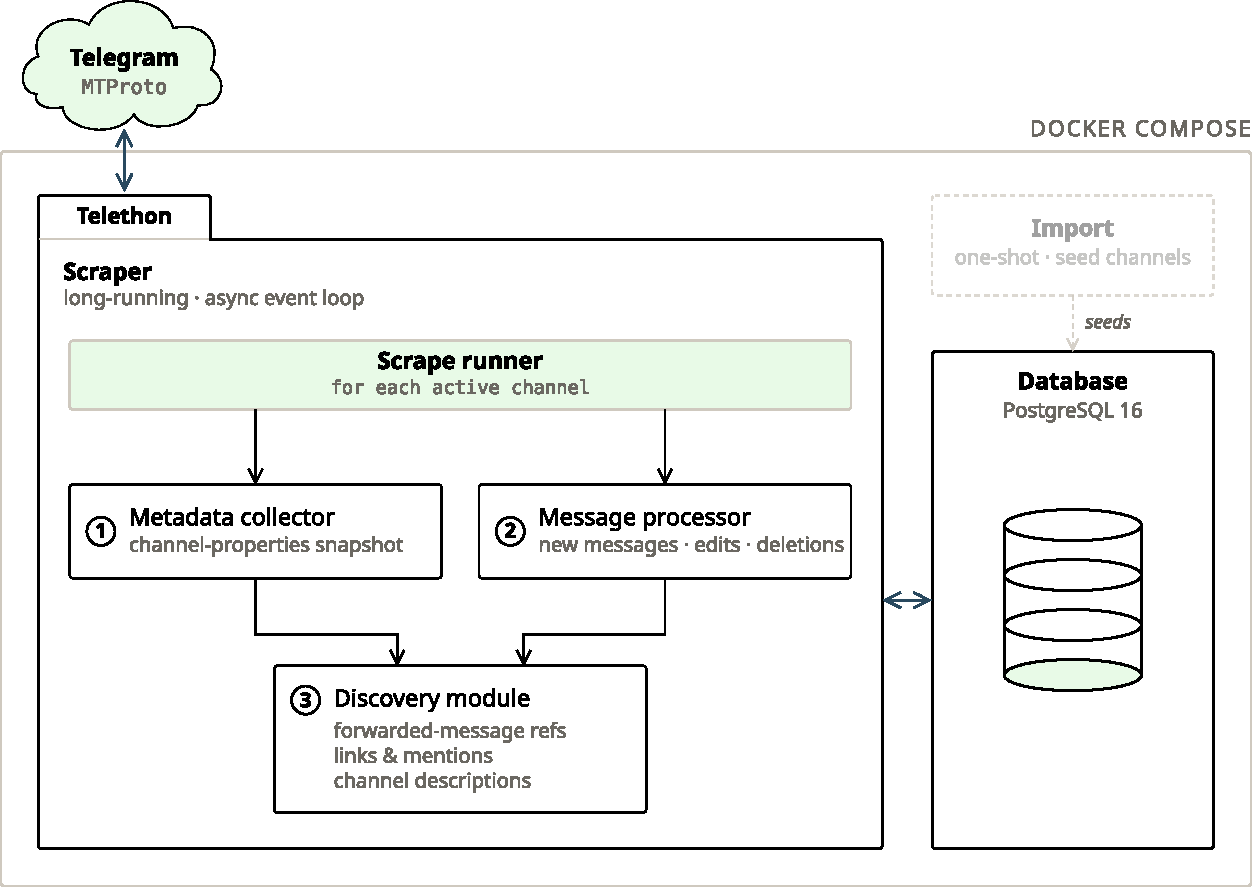
\includegraphics[width=\textwidth]{figures/architecture}
\caption[System architecture overview.]{System architecture. The scrape runner orchestrates three subsystems per channel: a metadata collector, a message processor, and a discovery module. Telethon mediates all communication with Telegram's MTProto API; PostgreSQL stores the collected data. The application is packaged as three Docker Compose services: the database, a one-time import job, and the scraper.}
\label{fig:architecture}
\end{figure}

%----------------------------------------------------------------------
\section{System Architecture}
\label{sec:architecture}
%----------------------------------------------------------------------

The system is implemented in Python using the Telethon library~\cite{telethon2026} for communication with Telegram's MTProto API.
Data is stored in a PostgreSQL~16 database, and the entire application is deployed via Docker Compose with three services: the database, a one-time channel-import job, and the scraper itself.

The scraper is structured as an asynchronous application built on Python's \texttt{asyncio} event loop.
At the top level, a \emph{scrape runner} orchestrates a continuous loop of crawl runs.
Each run iterates over the current set of active channels, and for each channel the runner invokes three subsystems in sequence: (1)~a \emph{metadata collector} that takes a snapshot of the channel's current properties, (2)~a \emph{message processor} that fetches new messages, detects edits, and identifies deletions, and (3)~a \emph{discovery module} that extracts references to previously unseen channels from forwarded messages, in-text links, and channel descriptions.

Communication with the Telegram API is subject to strict rate limits.
The scraper handles \texttt{FloodWaitError} responses by sleeping for the server-requested duration, and configurable jittered delays are inserted between API calls and between channels to reduce the likelihood of triggering rate-limit penalties.

%----------------------------------------------------------------------
\section{Telegram API and Client Library}
\label{sec:tools}
%----------------------------------------------------------------------

Telegram exposes two officially supported interfaces, and the choice between them constrains every subsequent design decision.

The \emph{Bot API}\footnote{\url{https://core.telegram.org/bots/api}} is a high-level HTTP-based interface designed for chatbot development.
It permits reading messages from groups or channels where the bot has been explicitly added, but it does not support historical message retrieval or channel discovery, ruling it out for large-scale public-channel crawling.

The \emph{MTProto API}\footnote{\url{https://core.telegram.org/api}} is Telegram's native binary protocol.
It exposes the full range of client functionality (channel search, message iteration with offset-based pagination, metadata retrieval, and entity resolution), making it the interface of choice for research-oriented scraping.
However, the MTProto API requires an authenticated \emph{user} session and is subject to strict rate limits; excessive request volumes can trigger temporary or permanent account restrictions.
We adopt MTProto despite the account-ban risk because the only alternative (the Bot API) cannot iterate the message history of a channel the bot has not been added to, and channel operators in the wild do not add third-party bots. MTProto is therefore not a preference but the only research-viable interface, and every prior dataset reviewed in Section~\ref{sec:telegram-datasets} reached the same conclusion. The risk is mitigated operationally by a dedicated secondary account and the rate-limit handling described in Section~\ref{sec:robustness}.

Two Python client libraries exist for the MTProto protocol: \textbf{Telethon}~\cite{telethon2026} and \textbf{Pyrogram}~\cite{pyrogram2024}.
Table~\ref{tab:tool-comparison} compares these alongside two other tools that are sometimes mentioned in the context of Telegram data collection but are not suitable for large-scale channel scraping.

\textbf{Telethon} is the most widely used Python MTProto library.
It provides an asynchronous abstraction over the raw protocol, supporting operations such as \texttt{iter\_messages}, \texttt{get\_messages}, and \texttt{get\_entity} that form the backbone of most Telegram scrapers in the literature~\cite{baumgartner2020,lamorgia2025,blas2025,propaganda2025}.
Telethon's \emph{takeout session} feature wraps requests in a mode that Telegram treats with relaxed flood limits, which is critical when iterating through hundreds of thousands of channels.
The library also caches entity access hashes in a local SQLite session file, eliminating redundant username-resolution calls on subsequent crawl runs.

\textbf{Pyrogram} offers a similar feature set with a more object-oriented API, but its maintenance status is the decisive concern: at the time of writing, no new release has appeared on PyPI in over 12~months and the GitHub repository shows no recent activity~\cite{pyrogram2024}.
For a long-running scraping project, an unmaintained MTProto library is a serious risk, as Telegram periodically updates its API layer and a library that does not track these changes will eventually fail to connect.
Pyrogram also lacks takeout session support, meaning the scraper cannot request relaxed flood limits for bulk export.

Two other tools warrant brief mention.
\textbf{telegram-export}~\cite{telegramexport2020} is an archived, unmaintained command-line tool (built on Telethon) designed for personal chat backup rather than channel discovery.
\textbf{python-telegram-bot}~\cite{pythontelegrambot2026} wraps the HTTP Bot~API, which cannot browse public channels or iterate their message histories, making it unsuitable for this use case.

\begin{table}[htbp]
\centering
\caption{Comparison of Python tools for Telegram data collection.}
\label{tab:tool-comparison}
\small
\begin{tabular}{@{}lcccc@{}}
\toprule
 & \textbf{Telethon} & \textbf{Pyrogram} & \textbf{telegram-export} & \textbf{PTB} \\
\midrule
Protocol        & MTProto & MTProto & MTProto & Bot API \\
Maintained      & Yes     & No      & No (archived) & Yes \\
Takeout support & Yes     & No      & No      & N/A \\
Licence         & MIT     & LGPL-3.0 & MPL-2.0 & LGPL-3.0 \\
Academic use    & Extensive & Occasional & None & None \\
\bottomrule
\end{tabular}
\end{table}

Our scraper is built on Telethon and inherits its rate-limit handling, including automatic sleep on \texttt{FloodWaitError} responses. All observations of API behaviour reported in this chapter (for example, the scoping semantics of \texttt{result.total} discussed in Section~\ref{sec:combined-pass}) were made against Telethon as pinned in the project's \texttt{pyproject.toml} at the time of data collection.

%----------------------------------------------------------------------
\section{Storage Back-End}
\label{sec:storage}
%----------------------------------------------------------------------

The storage back-end has to support the two workloads this system was designed for: bursty bulk inserts during crawl runs (hundreds of thousands of channels, hundreds of millions of messages, with append-only metadata and edit-history snapshots) and analytical queries for downstream study (temporal aggregations, forwarding-graph traversals, cross-channel joins). We do not claim these are the workloads of all Telegram scrapers; they are the workloads of \emph{this} scraper, and the back-end choice is justified against them. The two workloads do not necessarily run simultaneously: offline analyses can be performed on a static snapshot after a crawl run completes. However, a back-end that supports both concurrently on a single machine simplifies deployment and enables online monitoring or incremental analyses alongside the scraper without the overhead of exporting to a secondary system. We surveyed four candidate systems before settling on PostgreSQL; the comparison is summarized in Table~\ref{tab:db-comparison}.

\textbf{PostgreSQL}~\cite{postgresql2026} is a mature relational database with strong ACID guarantees, native JSONB support, and a rich indexing ecosystem (B-tree, GIN, GiST). Its \texttt{COPY} interface sustains the scraper's bulk-insert throughput, while its query planner, window functions, and recursive CTEs make temporal aggregations and forwarding-chain traversals expressible in standard SQL. The extension ecosystem (e.g., \texttt{pg\_trgm} for fuzzy text, pgvector for embedding-based similarity) provides a growth path without migrating to a different system.

\textbf{MongoDB}~\cite{mongodb2026} is the document store used in the original TGDataset paper~\cite{lamorgia2025}. Its schema-less model maps naturally onto the dict-like objects returned by Telethon, and GridFS offers a built-in mechanism for storing large binary files. However, the analytical workload is its weak point: aggregation pipelines are harder to write and optimize than equivalent SQL, and \texttt{\$lookup}-based cross-collection joins do not benefit from the same planner optimizations as relational joins. More critically, a nested schema that embeds all messages of a channel inside a single document would quickly exceed the 16\,MB BSON document size limit; promoting messages to their own collection recreates a relational structure but without referential integrity or standard SQL.

\textbf{SQLite}~\cite{sqlite2026} offers zero-configuration, single-file storage and is attractive for its portability, but it permits only one writer at a time. This would cause scraping and concurrent analytical queries to block one another, and its performance at the 500\,M-message scale degrades without manual partitioning across multiple database files. SQLite remains useful as a format for distributing read-only dataset snapshots, but not as the primary store.

\textbf{DuckDB}~\cite{duckdb2019} is an in-process columnar analytical engine with vectorized execution, making it extremely fast for full-table scans and aggregations. It is, however, designed for bulk-load-then-query patterns rather than for the steady stream of inserts characteristic of a long-running scraper: it has no concurrent-write support and costly \texttt{UPDATE}/\texttt{DELETE} operations. It is well suited as an optional analytical companion (its \texttt{postgres\_scanner} extension can query a live PostgreSQL instance), but not as the ingestion path.

We therefore adopt PostgreSQL~16 as the primary store. PostgreSQL is acknowledged to be slower than DuckDB for pure analytical scans and heavier to operate than SQLite; we accept both trade-offs because our workload mixes steady ingestion with concurrent reads, which is the pattern PostgreSQL's MVCC concurrency model is designed for. The relational model captures channels, metadata snapshots, messages, and edit histories as separate-but-related entities linked by foreign keys, and the remaining bottleneck (analytical speed) is addressable by attaching DuckDB via \texttt{postgres\_scanner} for ad-hoc analysis without changing the ingestion path. The schema that realizes these choices is detailed in Section~\ref{sec:schema}.

\begin{table}[htbp]
\centering
\caption{Comparison of candidate storage back-ends.}
\label{tab:db-comparison}
\small
\begin{tabular}{@{}lccc@{}}
\toprule
 & \textbf{PostgreSQL} & \textbf{MongoDB} & \textbf{SQLite} \\
\midrule
Bulk write throughput   & Excellent (\texttt{COPY}) & Good            & Fair           \\
Concurrent read/write   & Full MVCC                 & Full MVCC       & Single writer  \\
Analytical query speed  & Good                      & Mediocre        & Fair           \\
SQL support             & Full                      & None (MQL)      & Full           \\
Graph/recursive queries & Recursive CTEs            & \texttt{\$graphLookup} & Recursive CTEs \\
500\,M+ row viability   & Proven                    & Proven          & Strained       \\
Operational complexity  & Moderate                  & Moderate        & Zero           \\
\bottomrule
\end{tabular}
\end{table}

%----------------------------------------------------------------------
\section{Channel Discovery}
\label{sec:channel-discovery}
%----------------------------------------------------------------------

Channel discovery is built on snowball sampling, a chain-referral technique in which an initial set of seed entities expands iteratively by following social connections to discover previously unknown entities~\cite{goodman1961}.
Telegram's forwarding mechanism makes this technique particularly well suited to channel discovery: there is no centralized directory of public channels, but forwarded messages carry explicit references to their source channels, providing a built-in traversal link.
The known biases and limitations of snowball sampling as applied here are discussed in Section~\ref{sec:limitations}.

Starting from a user-provided set of seed channels, the scraper discovers new channels through three sources:

\begin{enumerate}
    \item \textbf{Forwarded messages.} When a message is forwarded from another channel, Telegram's API includes the source channel's numeric identifier in the \texttt{fwd\_from} field.
    These identifiers can be inserted into the database directly without additional API calls.

    \item \textbf{Links and mentions in message text.} The scraper applies regular expressions to extract \texttt{t.me/} URLs and \texttt{@username} mentions from the body of each message.
    A set of known false-positive paths (e.g., \texttt{joinchat}, \texttt{addstickers}, \texttt{share}) is filtered out.

    \item \textbf{Channel descriptions.} The same link-extraction logic is applied to each channel's ``about'' text, which is retrieved as part of the metadata snapshot.
\end{enumerate}

\begin{figure}[htbp]
\centering
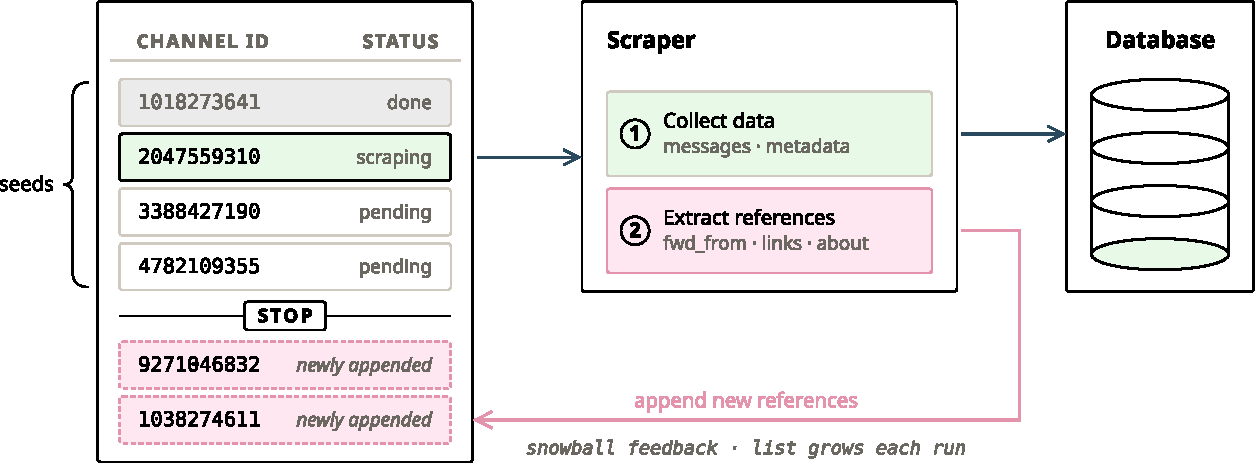
\includegraphics[width=\textwidth]{figures/snowball}
\caption[Snowball discovery loop.]{Snowball discovery loop. The scraper reads the next pending channel from the database-backed list, records its messages and metadata, extracts references to previously unseen channels from forwards, in-text links, and channel descriptions, and appends them to the list. Newly appended entries (below the run's STOP marker) are scraped on the following run.}
\label{fig:snowball}
\end{figure}

Forward-discovered channel IDs are registered in the database immediately, since Telethon provides the numeric identifier at no extra cost.
Username-based discoveries, by contrast, require a \texttt{contacts.ResolveUsername} API call to map the username to a channel ID.
The scraper implements a batched resolution mechanism: discovered usernames are queued in an \texttt{unresolved\_references} table (Section~\ref{sec:schema}) and resolved with doubled inter-request delays, while permanently invalid usernames (e.g., deleted or private channels) are marked and excluded from future attempts.

In practice, however, username resolution is disabled in our deployment because Telegram imposes strict rate limits on \texttt{contacts.ResolveUsername}.
The daily limit is documented at roughly 200 calls~\cite{tginfolimits}, and exceeding it triggers a \texttt{FLOOD\_WAIT\_X} error~\cite{telegramapierrors} with mandatory wait times that can reach 24 hours.
For a continuously running scraper that already consumes its rate budget on message retrieval, spending part of that budget on username resolution is impractical.
Channel discovery therefore relies exclusively on forwarded-message identifiers, which the API provides at no additional cost.
Disabling username resolution introduces a known sampling bias: channels that are only reachable through \texttt{@}-mentions or \texttt{t.me/} links, without ever being forwarded, are under-sampled. We accept this bias because the alternative (spending the rate-limit budget on resolution calls) would halt message collection outright, and because forwarded-message references are empirically the dominant discovery channel on our deployment, as reported in Chapter~\ref{chap:results}. The bias is revisited in the Limitations section of Chapter~\ref{chap:results}.

Because channels discovered during a run are added to the database but not to the current run's channel list, the snowball expansion takes effect on the \emph{next} run.
This design avoids unbounded growth of a single run and ensures that the channel list for each run is fixed at the start, simplifying crash recovery (Section~\ref{sec:robustness}).

Figure~\ref{fig:snowball} summarizes the resulting feedback loop: each run iterates over a channel list drawn from the database; for every channel the scraper collects messages and metadata, extracts references to previously unseen channels, and appends them to the list for use by the next run.

%----------------------------------------------------------------------
\section{Database Schema}
\label{sec:schema}
%----------------------------------------------------------------------

The database schema is designed around four requirements: preserving Telegram's native identifiers, supporting longitudinal metadata tracking, recording message edit histories, and enabling crash-safe incremental collection.
Eight tables, whose relationships are summarized in Table~\ref{fig:erd}, serve three functional groups: channel identity and metadata, message storage and edit history, and operational bookkeeping.

\begin{figure}[htbp]
\centering
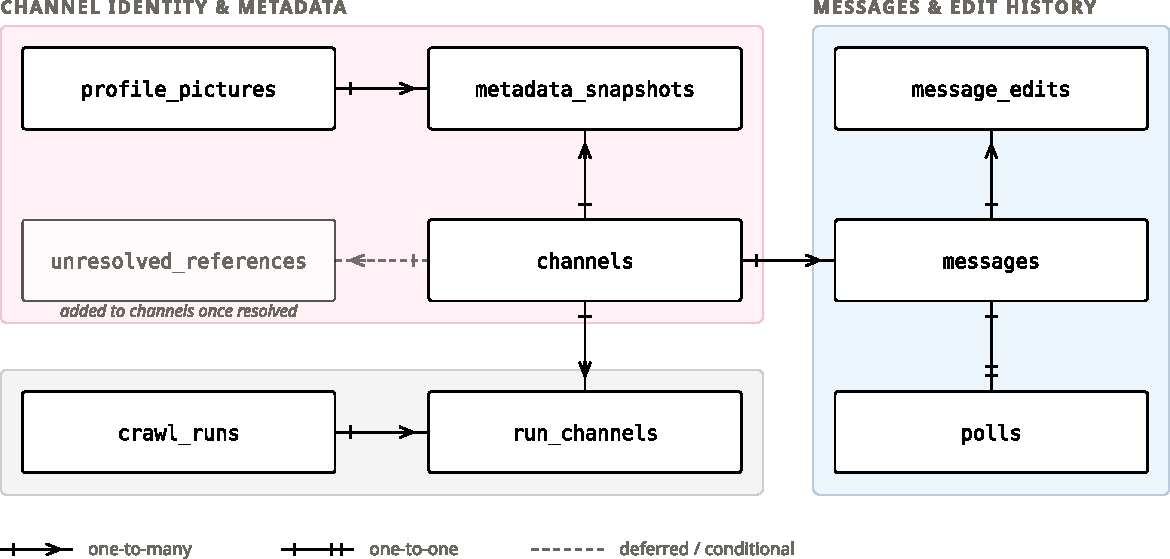
\includegraphics[width=\textwidth]{figures/erd}
\caption[Database schema entity-relationship diagram.]{Entity-relationship diagram of the database schema. Solid arrows denote one-to-many or one-to-one relationships (see legend); \texttt{unresolved\_references} (dashed border) is linked to \texttt{channels} conditionally, once a username has been resolved to a channel ID. Three functional groups are shaded: channel identity and metadata (top left), messages and edit history (right), and operational bookkeeping (bottom).}
\label{fig:erd}
\end{figure}

\subsection{Channel identity and metadata}

\paragraph{Channels.}
The \texttt{channels} table stores one immutable identity record per channel, keyed by Telegram's native signed 64-bit channel ID.
Each row records when the channel was created, when the scraper first encountered it, and how it was discovered (\texttt{seed}, \texttt{forward}, \texttt{mention}, \texttt{manual}, or \texttt{linked\_group}).
Three boolean flags support the scraping cycle: \texttt{is\_active} acts as a circuit breaker that disables a channel after a configurable number of consecutive failures, \texttt{initial\_pull\_complete} tracks whether the first full historical download has finished, and \texttt{needs\_recheck} is set before processing and cleared on success, surviving crashes to trigger a forced recheck on restart.
A \texttt{linked\_to\_channel\_id} foreign key records the parent for channels that serve as discussion groups.

\paragraph{Metadata snapshots.}
The \texttt{metadata\_snapshots} table stores one row for each channel on every crawl visit, forming the core of the longitudinal tracking.
Each snapshot captures the channel's public identity (username, title, description), its subscriber count, trust-related flags set by Telegram (scam, verified, restricted, fake), a reference to the active profile picture, and the linked discussion-group ID.
A dedicated \texttt{is\_private} flag marks snapshots recorded when the channel returned a \texttt{ChannelPrivateError}; in these rows all other fields are null.
By diffing consecutive snapshots one can detect name changes, description edits, subscriber growth or decline, profile-picture swaps, and transitions to or from private status.

\paragraph{Profile pictures.}
Channel profile pictures are stored in a content-addressable \texttt{profile\_pictures} table, keyed by the SHA-256 hash of the raw image bytes.
Each row also stores a 64-bit DCT-based perceptual hash and a 64-bit difference hash, enabling near-duplicate detection across channels.
Idempotent insertion (\texttt{ON CONFLICT DO NOTHING}) ensures that the same image is stored only once, even when multiple snapshots reference it.
Photo-change detection is optimized by comparing the \texttt{photo\_id} (a lightweight integer exposed by the API) between consecutive snapshots; the image bytes are downloaded only when a change is detected.

\subsection{Messages and edit history}

\paragraph{Messages.}
The \texttt{messages} table is the central fact table, keyed by the composite primary key \texttt{(channel\_id, message\_id)}.
Table~\ref{tab:messages} summarizes the information stored for each message, grouped thematically.
Columns are physically ordered by descending alignment size (8-byte, 4-byte, 1-byte, variable-length) to minimize PostgreSQL's inter-column padding overhead, which would otherwise waste approximately 7--8~bytes per row.
The variable-length columns (\texttt{text} for message bodies, \texttt{jsonb} for entities and reactions) keep PostgreSQL's default \texttt{EXTENDED} storage strategy. \texttt{EXTENDED} declares a column \emph{eligible} for compression and for out-of-line storage in the TOAST side-table; neither is applied until the row would otherwise exceed the tuple threshold (\texttt{TOAST\_TUPLE\_THRESHOLD}, roughly 2\,kB). Short messages therefore remain inline and uncompressed, while long ones are compressed first and moved out-of-line only if still too large. This behaviour matches our workload: most Telegram posts are short and cost nothing to read, while the rare long post does not bloat the main heap.

\begin{table}[htbp]
\centering
\caption{Information stored per message in the \texttt{messages} table, grouped by theme.}
\label{tab:messages}
\small
\begin{tabular}{@{}lp{8.5cm}@{}}
\toprule
\textbf{Group} & \textbf{What is stored} \\
\midrule
Timestamps      & Publication date, last edit date, and the time the message was first collected by the scraper. \\
Content         & Raw message text (PostgreSQL \texttt{text}), structured entities (URLs, mentions, formatting as JSONB), a media-type indicator, a service-action type for system messages such as channel creation or pin events, and a JSONB payload that preserves the action's constructor arguments for actions that carry one. Media files themselves are not downloaded: see the rationale below. \\
Authorship      & Poster's numeric user or channel ID and an optional author-signature string. \\
Engagement      & View count, forward count, reply count, pinned status, and per-emoji reaction counts (JSONB). \\
Forwarding      & Whether the message is a forward, the source channel ID and message ID, the original posting date, and a display name for hidden or deleted sources. \\
Threading       & Reply-to message ID, top-level thread ID, a comment-thread flag, and an album-grouping ID for multi-media posts. \\
Deletion        & A deleted flag and a timestamp recording when the deletion was detected (Section~\ref{sec:combined-pass}). Deleted rows are retained to preserve the historical record. \\
\bottomrule
\end{tabular}
\end{table}

Media files attached to messages (photos, videos, documents) are deliberately not downloaded. Storing media at dataset scale would additional storage, raises legal sensitivity around potentially copyrighted or illicit content, and is out of scope for a study whose primary unit of analysis is channel metadata and text. The stored media-type indicator is sufficient to reconstruct any media file on demand via the Telegram API, should a downstream study require it.

\paragraph{Message edits.}
The \texttt{message\_edits} table preserves previous versions of edited messages.
When an edit is detected, the current content of the \texttt{messages} row (text, entities, media flag, and media type) is copied here before the row is overwritten with the new version.
The \texttt{messages} table therefore always holds the latest version, while the full edit history is available by joining with \texttt{message\_edits} and ordering by the \texttt{captured\_at} timestamp.

\paragraph{Polls.}
Messages whose \texttt{media\_type} is \texttt{poll} are accompanied by a row in the \texttt{polls} table, keyed by the same \texttt{(channel\_id, message\_id)} composite key.
Each row stores the stable Telegram poll identifier, the question text and its formatting entities, and a JSONB \texttt{answers} array whose elements record option text, raw option bytes (base64-encoded), vote tallies, and, for quizzes, a flag indicating the correct answer.
Four boolean flags characterize the poll configuration: \texttt{is\_closed}, \texttt{is\_quiz}, \texttt{is\_multiple} (whether multiple answers may be selected), and \texttt{is\_public\_voters} (whether individual votes are visible to subscribers).
Optional fields capture the close schedule (\texttt{close\_period}, \texttt{close\_date}), the aggregate voter count, and the quiz explanation text (\texttt{solution}).
The table is latest-only: re-observation overwrites the mutable fields (tallies, \texttt{is\_closed}) in place and advances \texttt{captured\_at}, so the row always reflects the most recent snapshot rather than a full history of vote counts.

\subsection{Operational bookkeeping}

\paragraph{Crawl runs and run channels.}
The \texttt{crawl\_runs} table records every scraping or alignment run with its type, status, start and end timestamps, progress counters (channels attempted, channels completed, messages collected), and, for alignment runs, the cutoff timestamp.
A JSONB \texttt{config\_snapshot} column preserves the scraper's configuration at the time of each run for reproducibility.
The associated \texttt{run\_channels} table persists the ordered list of channels for each run, with a per-channel status (\texttt{pending}, \texttt{completed}, \texttt{partial}, or \texttt{error}). The \texttt{partial} status records that the channel was processed but its pull was interrupted by a sustained network outage; see Section~\ref{sec:robustness}.
Together, these two tables enable crash recovery: on restart the scraper queries for the most recent incomplete run, retrieves its pending channels, and resumes from where it left off.

\paragraph{Unresolved references.}
The \texttt{unresolved\_references} table queues usernames discovered via links and mentions that have not yet been resolved to channel IDs.
Each entry tracks the number of resolution attempts and the timestamp of the last attempt, implementing a retry-with-backoff strategy.
As noted in Section~\ref{sec:channel-discovery}, the resolution mechanism is not used in our deployment due to Telegram's rate limits on \texttt{contacts.ResolveUsername}; the table nonetheless records the discovered usernames for potential offline or manual resolution.

%----------------------------------------------------------------------
\section{Scraping Cycle}
\label{sec:scraping-cycle}
%----------------------------------------------------------------------

The scraper operates in a continuous loop of crawl runs, with the database as the single source of truth for which channels to process.

\paragraph{Run initialization.}
At the start of each run, the scraper queries the \texttt{channels} table for all rows where \texttt{is\_active = true}, creates a new entry in \texttt{crawl\_runs}, and persists the ordered channel list to \texttt{run\_channels}.
The list is built from two concatenated segments. The first segment contains all channels that have already been scraped in a previous run, kept in a fixed order that simply grows as new channels graduate into it. The second segment contains all channels not yet scraped (the seed set on the very first run, plus any references discovered since), and is shuffled at random before the start of the run.
Shuffling the unscraped segment matters because a single channel can contribute hundreds of new references in one visit (through forwards, in-text links, and its description); without randomization those references would be processed back-to-back, skewing the sample toward large or densely-connected forwarding graphs. Interleaving them with references discovered by other channels diffuses this locality.
Figure~\ref{fig:snowball-list} shows how this two-part structure evolves across successive runs: the ``seen'' prefix accumulates monotonically while each fresh batch of discovered references is shuffled before being appended.
The channel list is fixed for the duration of the run; channels discovered during processing are added to the database but only appear in subsequent runs.

\begin{figure}[htbp]
\centering
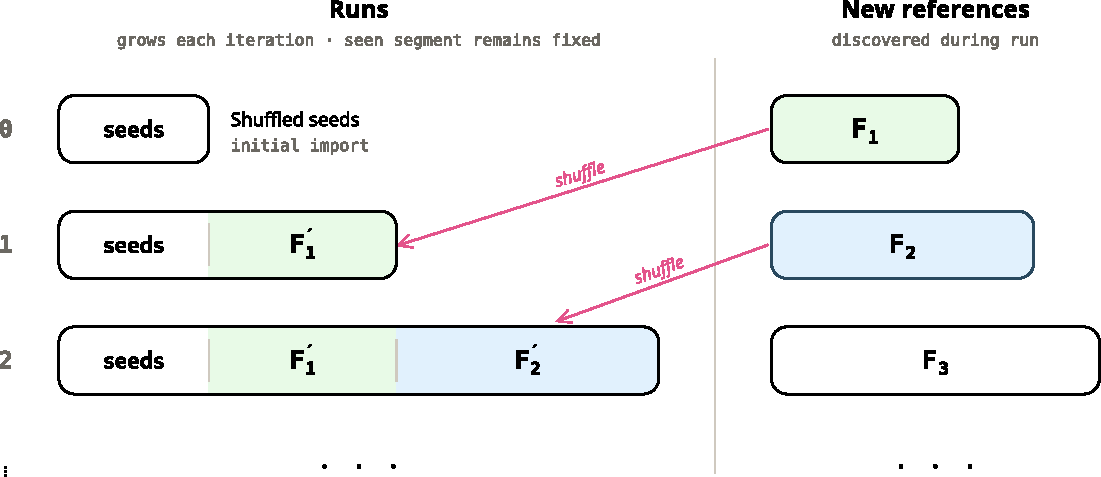
\includegraphics[width=\textwidth]{figures/snowball_list}
\caption[Scraping-list growth across runs.]{Evolution of the scraping list across successive runs. In run~0 the list contains only seeds, shuffled. After run~0, the seeds move into the fixed ``seen'' prefix and the new references $F_1$ discovered during the run are shuffled into the unscraped segment as $F'_1$ for run~1. This pattern repeats: the seen prefix grows monotonically while each fresh batch of discovered references is shuffled before being appended.}
\label{fig:snowball-list}
\end{figure}

\paragraph{Per-channel processing.}
For each channel, the scraper performs three steps:
\begin{enumerate}
    \item \textbf{Metadata snapshot.} A single \texttt{GetFullChannelRequest} API call retrieves the channel entity and its extended metadata, which is inserted as a new row in \texttt{metadata\_snapshots}.
    If the profile picture has changed (detected via \texttt{photo\_id} comparison), the new image is downloaded, hashed, and stored.

    \item \textbf{Message processing.} The combined pass described in Section~\ref{sec:combined-pass} fetches new messages, detects edits on previously stored messages, and identifies deletions.

    \item \textbf{Channel discovery.} Forward references and link-based usernames extracted during message processing, together with links from the channel description, are registered or queued for resolution.

    \item \textbf{Linked discussion group (conditional).} A broadcast channel can have an associated discussion group attached to it; messages posted by subscribers in that group, threaded under a broadcast post, are what Telegram exposes as ``comments'' on the post. If the parent's metadata snapshot reports such a linked group and comment collection is enabled, the group is recorded in \texttt{channels} with source \texttt{linked\_group} and a back-pointer to the parent. The same three steps above are then applied to the linked group as part of the same per-channel iteration, sharing the parent's run identifier and (during alignment) cutoff timestamp. The back-pointer marks the linked group as a child of an already-queued channel, so it is excluded from the regular scrape queue and is visited only as part of its parent's turn, which preserves the channel/group pair as a single unit of work.
\end{enumerate}

After each channel completes, its \texttt{run\_channels} row is updated from \texttt{pending} to \texttt{completed} (or \texttt{partial} or \texttt{error}), and the run-level counters are incremented.
If a shutdown signal is received mid-iteration, the run is marked as \texttt{interrupted} and the remaining channels are left as \texttt{pending} for resumption.

\paragraph{Inter-run behavior.}
Runs repeat indefinitely.
Each new run sees the full, up-to-date channel list, including any channels discovered during previous runs.
Before starting a fresh run, the scraper checks for incomplete runs from prior sessions and resumes them first (Section~\ref{sec:robustness}).

%----------------------------------------------------------------------
\section{Combined Pass: New Messages, Edit Detection, and Deletion Detection}
\label{sec:combined-pass}
%----------------------------------------------------------------------

The three core message-level operations (fetching new content, detecting edits, and identifying deletions) are performed together in a single combined pass per channel, minimizing redundant API calls.
The pass branches based on whether deletions are detected.

\subsection{Setup}
\label{sec:combined-setup}

For each channel, two values are derived from the \texttt{messages} table at query time:
\begin{itemize}
    \item \texttt{highest\_id}: the maximum \texttt{message\_id} stored for this channel.
    \item \texttt{message\_count}: the number of non-deleted messages whose \texttt{message\_id} lies in the range $[0, \texttt{highest\_id}]$.
\end{itemize}

\begin{figure}[htbp]
\centering
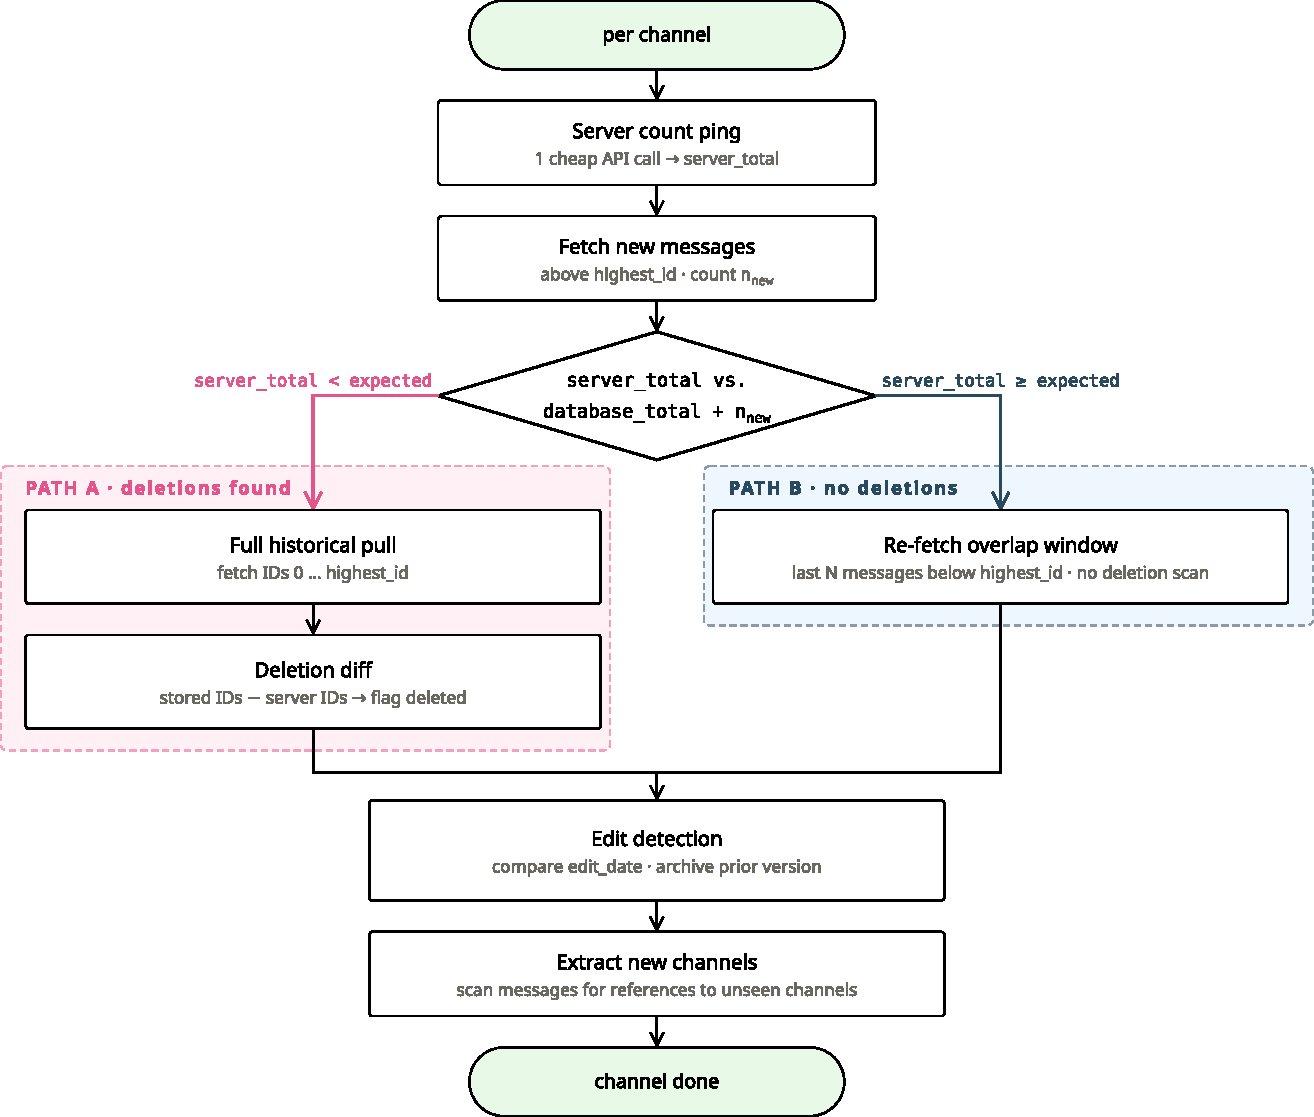
\includegraphics[width=\textwidth]{figures/combined-pass}
\caption[Combined-pass flowchart.]{Combined pass for a single channel. A cheap preliminary ping yields \texttt{server\_total}; after the new-message fetch, the comparison against $n_{\text{expected}}$ branches into Path~A (full historical pull with deletion diff) or Path~B (re-fetch of the overlap window). Edit detection is a shared subroutine: both paths feed every fetched message into the same \texttt{edit\_date} comparison.}
\label{fig:combined-pass}
\end{figure}

If \texttt{highest\_id} is null (no messages have ever been collected), the scraper performs a full initial pull, paginating through all messages from newest to oldest and committing each batch to the database as it arrives.

\subsection{Deletion count check}

A single cheap API call retrieves the server-reported total message count:
\begin{lstlisting}[language=Python]
result = await client.get_messages(entity, limit=0)
server_total = result.total
\end{lstlisting}

We observed empirically that \texttt{result.total} always returns the \emph{full} channel message count regardless of any \texttt{min\_id} or \texttt{max\_id} parameters: passing \texttt{max\_id=100}, \texttt{max\_id=10000}, or no bound at all yields the same scalar.
The count cannot therefore be scoped to a historical range, and new messages must be fetched and counted before the comparison can be made.
The flip side of this constraint is what makes the strategy work: because \texttt{server\_total} is channel-global, a single equality between \texttt{server\_total} and the locally derived expected count rules out deletions \emph{anywhere} in the channel, not just above some cutoff. This is the guarantee that justifies the cheap path~B described next.

\subsection{Branching logic}

After fetching new messages (those with IDs above \texttt{highest\_id}) and counting them as $n_{\mathrm{new}}$, the expected count is computed as $n_{\mathrm{expected}} = \texttt{message\_count} + n_{\mathrm{new}}$.
The pass then branches:

\paragraph{Path A: deletions detected ($\texttt{server\_total} < n_{\mathrm{expected}}$).}
At least one message has been removed somewhere in $[0, \texttt{highest\_id}]$, and the count check by itself cannot say where. The number of missing messages, however, is known exactly: because \texttt{server\_total} is channel-global, the deficit $\Delta = n_{\mathrm{expected}} - \texttt{server\_total}$ is precisely how many stored IDs the server no longer returns. Locating them in full requires a historical pull that re-fetches every message from ID~0 to \texttt{highest\_id}. On a large channel this sweep is costly, and running it on every visit that detects even a single deletion would dominate the per-channel API cost.

Under the assumption that most deletions are recent, Path~A first attempts a cheap recent-window scan before committing to the full sweep. It re-fetches only the same overlap window of $N$ messages below \texttt{highest\_id} that Path~B uses for edits, and diffs the stored IDs within that window against the IDs the server returns for it. If the number of in-window deletions is at least $\Delta$, then every missing message lies inside the window: the entire deficit is accounted for, none can lie below it, and the full pull is skipped. Only when fewer than $\Delta$ deletions are found in the window, leaving part of the deficit unexplained, does the scraper fall back to the full historical pull from ID~0.

The threshold is ``at least $\Delta$'' rather than ``exactly $\Delta$'' by design. A deletion occurring inside the window between the count ping and the window scan can push the in-window count above $\Delta$; those extra IDs are genuinely absent from the window, which was scanned in full, so marking them and skipping remains correct. The test is unsafe only in the opposite direction, when $\Delta$ understates the true number of deletions, and that can happen only if $n_{\mathrm{new}}$ was undercounted by an interrupted new-message fetch. The fast path is therefore attempted only when that fetch completed cleanly and the channel's stored history is already known to be contiguous ($\texttt{initial\_pull\_complete} = \text{true}$); a forced crash-recovery recheck (Section~\ref{sec:robustness}), where the counts cannot be trusted, bypasses the window scan and goes straight to the full historical pull.

Whichever scan runs, deletion handling is identical: IDs present in the database but absent from the scan are flagged as deleted (the rows are retained with \texttt{is\_deleted = true} and a \texttt{deleted\_at} timestamp, preserving the historical record). Edit detection is piggybacked on the fetched messages: for each that already exists in the database, the \texttt{edit\_date} is compared against the stored value, and edits are archived. On a successful fast path the overlap window is edit-scanned exactly as in Path~B.

\paragraph{Path B: no deletions ($\texttt{server\_total} \geq n_{\mathrm{expected}}$).}
Only an overlap window of $N$ messages below \texttt{highest\_id} is re-fetched (where $N$ is configurable, defaulting to~100).
These messages are checked for edits, but no deletion scan is performed: the channel-global equality already established in Section~\ref{sec:combined-pass} mathematically covers every ID in $[0, \texttt{highest\_id}]$, so re-verifying any subset of that range would be redundant. The overlap window exists purely to surface edits, which the count check cannot detect because edits do not change the message total.

The count-based heuristic has a known blind spot: if exactly as many messages are deleted as are newly posted between two visits, \texttt{server\_total} will equal $n_{\mathrm{expected}}$ and the deletion will be silently missed until a subsequent visit restores the imbalance. We accept this because the only alternative is a full-history pull on every visit. Such a pull would multiply the per-channel API cost by several orders of magnitude and make continuous crawling inefficient. Two further limitations follow from the same trade-off and are revisited in Section~\ref{sec:limitations}. First, Path~B sees no edits to messages older than the overlap window until that channel happens to enter Path~A. Second, a benign race between the count ping and the new-message pull can occasionally inflate $n_{\mathrm{expected}}$ enough to trigger a redundant (but non-corrupting) Path~A run. A related but distinct issue during alignment runs, where the cutoff timestamp applies only to the new-message fetch and not to the count ping, is discussed in Section~\ref{sec:alignment}.

\subsection{Edit detection logic}

Whenever a message is fetched (in either path), its \texttt{edit\_date} is compared against the version stored in the database:
\begin{itemize}
    \item If the stored \texttt{edit\_date} is null and the fetched one is set, or the fetched \texttt{edit\_date} is strictly newer, an edit is recorded.
    \item The current version in \texttt{messages} is copied to \texttt{message\_edits} (preserving the pre-edit content), and the \texttt{messages} row is then updated with the new content.
\end{itemize}
No additional API calls are needed: edit detection piggybacks entirely on the message fetches already required for deletion checking and new-message collection.

%----------------------------------------------------------------------
\section{Alignment Snapshots}
\label{sec:alignment}
%----------------------------------------------------------------------

A key challenge in longitudinal dataset construction is ensuring temporal consistency: when crawling thousands of channels sequentially, channels processed early in a run reflect data from a different point in time than those processed later.
Alignment snapshots address this by bringing all channels to a common cutoff timestamp.

\subsection{Trigger}

An alignment snapshot can be triggered in two ways: automatically, when a configurable interval (e.g., 30~days) has elapsed since the last alignment, or manually, by sending a \texttt{SIGUSR1} signal to the scraper process.
In both cases, the current scrape run is interrupted and marked accordingly, and a cutoff timestamp $t_c$ is set to the current time.

\subsection{Alignment processing}

A new crawl run of type \texttt{alignment\_snapshot} is created with \texttt{cutoff\_timestamp} = $t_c$.
The alignment iteration processes all channels that have been fully scraped at least once (\texttt{initial\_pull\_complete = true}).
For each channel, the same combined pass as a regular scrape is executed (Section~\ref{sec:combined-pass}), with one modification: new messages are fetched only up to $t_c$ by setting Telethon's \texttt{offset\_date} parameter.
This ensures that every channel's message history is complete up to the same point in time.
Alignment is \emph{eventually consistent}, not instantaneous: the alignment run itself takes time to traverse all channels, and during that traversal the metadata of channels processed earlier continues to drift. What the cutoff timestamp guarantees is that every channel's message stream is captured up to the same $t_c$; it does not guarantee that the metadata snapshots across channels were taken at the same wall-clock moment. This is an inherent limit of sequential single-machine scraping rather than a shortcoming of the alignment protocol, and the drift is bounded by the duration of one alignment cycle.

\paragraph{Path selection under the cutoff.}
The cutoff $t_c$ is propagated into the new-message fetch via \texttt{offset\_date}, but not into the preliminary count ping, which cannot be scoped to a historical range (Section~\ref{sec:combined-pass}). During alignment, therefore, \texttt{server\_total} reports the channel-global count at the moment the channel's turn arrives, while $n_{\mathrm{new}}$ stops at $t_c$. Any message posted in the interval $[t_c, \text{now}]$ inflates \texttt{server\_total} without inflating $n_{\mathrm{expected}}$, so the cheap check enters Path~A only when the number of genuine deletions exceeds the number of post-cutoff posts. This widens the intra-request race described in Section~\ref{sec:combined-pass} from the gap between two API calls (seconds) to the gap between the alignment trigger and the channel's turn (minutes to hours on a large channel list), and its effect is to \emph{mask} deletions rather than falsely signal them. Busy channels processed late in the alignment queue are therefore the most exposed. The asymmetry is tolerated because alignment is always followed by a fresh regular scrape (the post-alignment step described below), which runs without a cutoff and exercises an exact cheap check, so any deletion masked during alignment surfaces on the immediately following pass. Alignment also does not unconditionally force Path~A: the \texttt{needs\_recheck} flag is set on each channel as a crash-guard, but path selection reads its \emph{prior} value, so only channels whose flag was already set (for example, by an earlier crash) take Path~A regardless. Finally, the recent-window fast path within Path~A (Section~\ref{sec:combined-pass}) tests against this same understated $\Delta$, so during alignment it can skip the full pull while a deletion below the overlap window goes unmarked; like a fully masked deletion, it is recovered by the exact check on the immediately following regular scrape.

\begin{figure}[htbp]
\centering
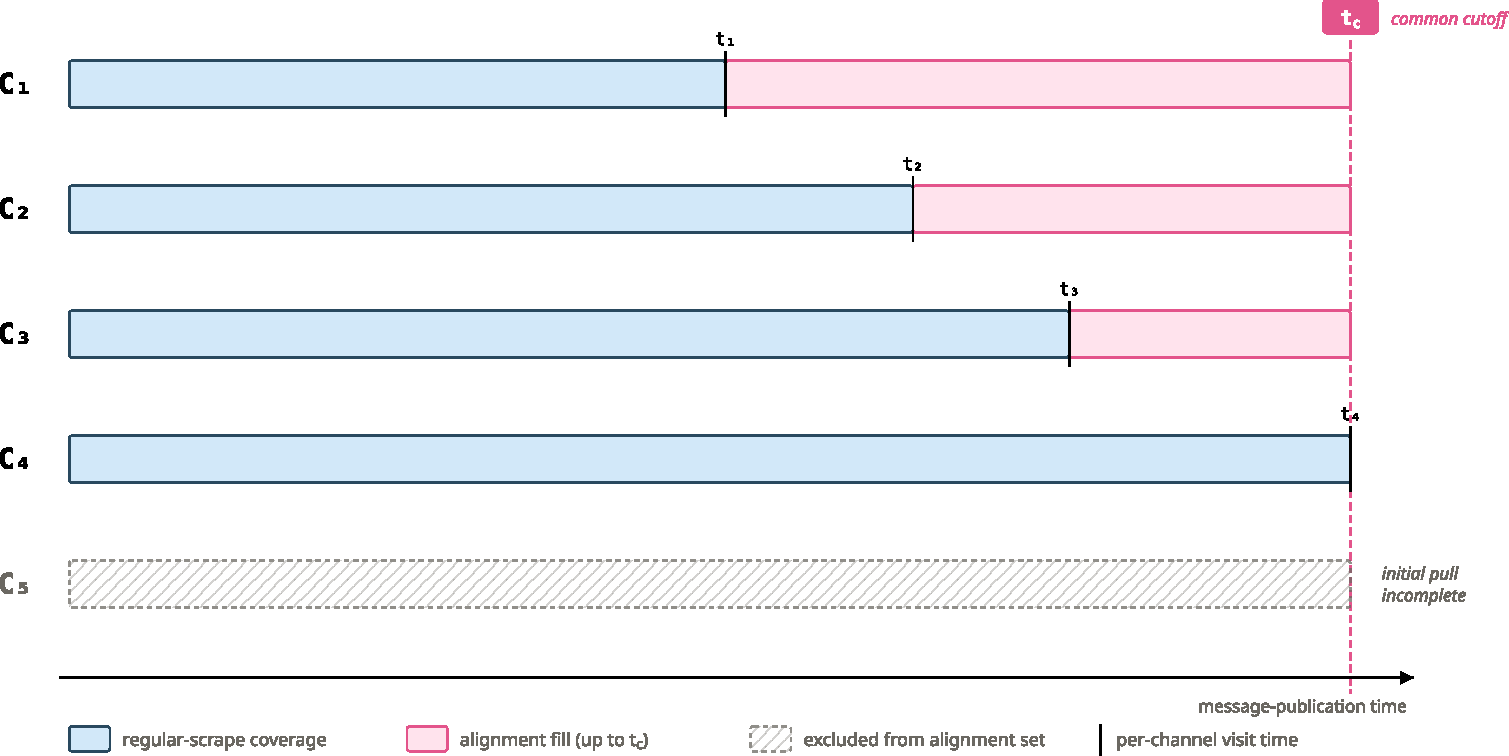
\includegraphics[width=\textwidth]{figures/alignment}
\caption[Alignment data coverage.]{What alignment guarantees, shown as per-channel message-stream coverage. The horizontal axis is message-publication time (not scraper wall-clock). During a regular scrape each channel $C_i$ is visited at a different moment $t_i$, so its data ends at a different point (blue segments). The alignment run then fills, for every channel with \texttt{initial\_pull\_complete\,=\,true}, the gap from $t_i$ up to the common cutoff $t_c$ (orange segments), so every channel's message history is complete up to the same point in time. Channels that have not completed their initial pull ($C_5$ here) are excluded from the alignment set (\texttt{get\_scraped\_channel\_ids} returns only fully scraped channels) and wait for a subsequent regular run before any future alignment can include them.}
\label{fig:alignment}
\end{figure}

\subsection{Post-alignment}

Once the alignment iteration completes, the alignment flag is cleared and a regular scrape run resumes with the full channel list, including any channels discovered during both the interrupted scrape and the alignment itself.

%----------------------------------------------------------------------
\section{Robustness}
\label{sec:robustness}
%----------------------------------------------------------------------

The scraper is designed to run continuously over weeks or months, and must tolerate network failures, process crashes, and API errors without data loss or corruption.
Several mechanisms contribute to this goal.

\paragraph{Graceful shutdown.}
The scraper installs handlers for \texttt{SIGTERM} and \texttt{SIGINT}.
When a shutdown signal is received, an asyncio event is set that is checked between batches and between channels.
The current operation is allowed to finish, the active run is marked as \texttt{interrupted}, and the process exits cleanly.

\paragraph{Crash recovery.}
Recovery operates at two levels.
At the \emph{run level}, on startup the scraper marks any leftover \texttt{running} crawl runs as \texttt{interrupted} and queries for the most recent incomplete run.
If one is found, its pending channels are retrieved from \texttt{run\_channels} and processing resumes from there.
At the \emph{channel level}, two flags on the \texttt{channels} table provide fine-grained recovery.
The \texttt{initial\_pull\_complete} flag is set to \texttt{false} until the first full historical download finishes; if a crash occurs mid-pull, the next run detects the incomplete state and fetches only the missing older messages (below the lowest stored ID) rather than re-fetching everything.
The \texttt{needs\_recheck} flag is set before a channel is processed and cleared only after all processing (including channel-discovery resolution) succeeds; if it survives a crash, the channel receives a forced full historical check on the next run.

\paragraph{Per-page persistence.}
Messages are committed to the database in batches as they arrive from the API, rather than being buffered until the end of a channel.
This minimizes data loss on crash: at most one batch of messages (configurable, default 100) can be lost. Per-message transactions would eliminate even this bounded loss, but at a cost in transaction overhead; the batch-level bound is the accepted trade-off, and any lost batch is recovered on the next run because the same messages will be re-fetched as long as they sit above the stored \texttt{highest\_id}. The scraper is designed to run as a single process on a single machine; multi-instance or distributed scraping is explicitly out of scope.

\paragraph{Per-channel error handling.}
Private and invalid channels are handled differently.
When a channel returns a \texttt{ChannelPrivateError}, the scraper records a private snapshot (Section~\ref{sec:schema}) and moves on without incrementing the error counter, since a channel that has become private may later be made public again.
For other failures (e.g., deleted or temporarily unavailable channels), the error is logged and a \texttt{consecutive\_errors} counter is incremented.
The counter resets on success; when it reaches a configurable threshold (default~2), the channel is deactivated (\texttt{is\_active = false}), preventing further wasted API calls.

\paragraph{Connection resilience.}
Before processing each channel, the scraper checks whether the Telegram client connection is still alive and reconnects if necessary.
Message iteration is protected by a per-message timeout: if no message arrives within 60~seconds, the iterator is abandoned with a partial batch rather than blocking indefinitely.
When such a timeout fires, the scraper does not advance to the next channel. Instead it parks on the current channel, force-reconnects the Telegram client, probes the API with a lightweight RPC to confirm the connection is actually live, and retries the pull in place. Retries use an exponentially growing backoff capped at a few minutes, and are repeated up to a configurable attempt cap that, at the default backoff schedule, spans roughly a full day of downtime. Each retry resumes from the partial state already on disk via the \texttt{initial\_pull\_complete} machinery (Section~\ref{sec:schema}), so progress is monotone across attempts. If the attempt cap is reached without recovery, the channel's \texttt{run\_channels} row is recorded as \texttt{partial} (rather than \texttt{completed} or \texttt{error}) and its \texttt{needs\_recheck} flag is left set, so the next run revisits it and finishes the pull.

\paragraph{Rate-limit handling.}
\texttt{FloodWaitError} responses from the Telegram API cause the scraper to sleep for the server-requested duration plus a small buffer.
During username resolution, a flood-wait sets a cooldown timestamp that suppresses further resolution attempts until the penalty period expires, preventing escalating rate-limit penalties.

%----------------------------------------------------------------------
\section{Deployment}
\label{sec:deployment}
%----------------------------------------------------------------------

The system is packaged as a Docker Compose application comprising three services.
The \textbf{database} service runs PostgreSQL~16 (Alpine), with the schema automatically applied from an initialization script on first start and data persisted in a named volume.
Version~16 is chosen over the latest major release for its maturity (several minor releases of accumulated bug fixes), its long community-support window (through November~2028), and the wider availability of compatible extensions and client libraries; none of the features introduced in subsequent major versions materially affect this workload.
The \textbf{import} service is a one-time job that populates the \texttt{channels} table with the active dataset's seed channel IDs, read from a seed file (one ID per line) whose path is supplied by an environment variable, with optional additional seeds passed inline through a second variable; it exits after completion and is not restarted. For the main corpus this seed file was the TGDataset channels~\cite{lamorgia2025}, in randomized order.
The \textbf{scraper} service runs the main application, configured via environment variables for API credentials, database connection, timing parameters (request delay, channel delay, jitter), batch size, overlap window, alignment interval, and error thresholds.
The Telethon session file, which stores the authenticated user session, is bind-mounted into the container to persist across restarts.

All configuration parameters are exposed as environment variables with documented defaults, allowing deployment-time tuning without code changes.
Table~\ref{tab:config} lists the principal parameters. The values shown in the \textit{Default} column are the values that were in use throughout data collection; no deployment-time overrides were applied, so any result reported in Chapter~\ref{chap:results} can be reproduced by running the system with these exact settings. Data collection ran from April to June 2026.

\begin{table}[htbp]
\centering
\caption{Principal configuration parameters and their defaults.}
\label{tab:config}
\small
\begin{tabular}{@{}llp{6.5cm}@{}}
\toprule
\textbf{Parameter} & \textbf{Default} & \textbf{Description} \\
\midrule
\texttt{REQUEST\_DELAY}     & 0.1\,s & Delay between API requests \\
\texttt{CHANNEL\_DELAY}     & 0.1\,s & Delay between channels \\
\texttt{DELAY\_JITTER}      & 0.3    & Proportional jitter applied to delays \\
\texttt{BATCH\_SIZE}        & 100    & Messages buffered before database write \\
\texttt{MESSAGE\_OVERLAP}   & 100    & Window below \texttt{highest\_id} re-checked for edits (Path~B) and scanned for recent deletions (Path~A fast path) \\
\texttt{ALIGNMENT\_INTERVAL}& 30\,d  & Auto-alignment interval (0 = disabled) \\
\texttt{MAX\_CONSECUTIVE\_ERRORS} & 2 & Failures before channel deactivation \\
\texttt{ENABLE\_LINK\_DISCOVERY} & false & Resolve \texttt{t.me/} links and \texttt{@}-mentions during discovery \\
\texttt{SCRAPE\_COMMENTS}    & true & Collect linked discussion groups alongside their parent channel \\
\bottomrule
\end{tabular}
\end{table}

%----------------------------------------------------------------------
\section{Ethical Considerations}
\label{sec:ethics}
%----------------------------------------------------------------------

The data-collection methodology described above was designed under two self-imposed constraints that bear directly on the ethical posture of the project: only publicly broadcast content is collected, and Telegram's published rate limits are respected rather than circumvented.

\paragraph{Public-channel scope.}
The unit of collection is restricted to public channels, defined here as channels that are reachable through Telegram's built-in search or through a public \texttt{t.me/} URL without an invitation link. No private chats, private groups, or user-level (one-to-one) messages are ever fetched; channels that transition to a private state are recorded as private and the scrape moves on without retrieving their content (Section~\ref{sec:robustness}). Public channels function as one-to-many broadcasting media analogous to public social-media feeds (Chapter~\ref{chap:background}), and their content is accessible to any Telegram user without subscribing or being granted access. Collected metadata is similarly restricted to each channel's public identity (username, title, public description, public subscriber count, and Telegram-assigned flags such as scam, verified, restricted, and fake). Media files attached to messages are not downloaded (Section~\ref{sec:schema}); only the media-type indicator is stored, which avoids retaining potentially sensitive imagery, audio, or video. Subscriber-level personal data (lists of who follows a channel, individual reactions, or per-user identifiers in broadcast messages) is not collected.

\paragraph{No circumvention of API limits.}
All communication with Telegram goes through the official MTProto API via Telethon (Section~\ref{sec:tools}). The scraper does not employ unofficial reverse-engineered endpoints, scraping of the web client, browser automation, or any other mechanism that bypasses the supported interface. Telegram's rate-limit signaling is treated as authoritative: \texttt{FloodWaitError} responses cause the scraper to sleep for the server-requested duration plus a small buffer (Section~\ref{sec:robustness}), and a cooldown timestamp suppresses subsequent username-resolution attempts during the penalty period rather than retrying through a side channel. Configurable jittered delays between requests and between channels (Table~\ref{tab:config}) keep the steady-state request rate below the documented thresholds. When a documented daily limit cannot be reconciled with the message-collection workload, we forfeit the affected feature rather than work around it: username-based channel discovery is disabled outright (Section~\ref{sec:channel-discovery}) to stay within the roughly 200-call daily ceiling on \texttt{contacts.ResolveUsername}~\cite{tginfolimits}, accepting the resulting sampling bias as a cost of remaining within the platform's limits.

\chapter{Dataset Analysis and Results}
\label{chap:results}

This chapter showcases what the scraper makes possible: it exercises the new collection layers on the corpus to show the kinds of analysis they open up, rather than presenting the dataset as a body of settled evidence. It is organised around the contributions claimed in the Introduction rather than around the data schema: each section delivers one of those contributions and traces it back to the collection mechanism that made it possible. Section~\ref{sec:res-corpus} characterises what the corpus actually is relative to other Telegram datasets, establishing the framing on which every later section rests. Section~\ref{sec:res-network} reconstructs the forward graph from the corpus and corrects several common misreadings of it. Section~\ref{sec:res-layers} is the core: it presents the three core capability layers (comments, edits, and deletions), of which edits and deletions are collected by no prior general-purpose Telegram corpus and comments only by the concurrent TeraGram~\cite{teragram2026}, together with per-platform restriction, a signal prior corpora left unexposed inside serialized message objects; it then gathers the supporting content layers (engagement, language, polls, and service actions) and a set of deliberate null results. Section~\ref{sec:res-war} exercises several of these layers at once on a single current-events showcase, the 2026 US/Israel--Iran war.

%======================================================================
\section{What the Corpus Is}
\label{sec:res-corpus}
%======================================================================

We crawled $12{,}065$ channels for messages, just $2.6\%$ of the $456{,}554$ channels the database registers. The crawled set is composed of a random subset of TGDataset's channels~\cite{lamorgia2025} plus their linked discussion groups where available; the remaining $97.4\%$ is a discovery frontier of channels that were referenced but never pulled (Section~\ref{sec:res-frontier}). The value of this dataset is therefore not breadth but \emph{per-channel depth}: the comments, edits, deletions, and metadata snapshots collected for the channels we did crawl. Table~\ref{tab:res-scalars} summarises the corpus and isolates the additive layers that distinguish it from prior work.

\begin{table}[htbp]
\centering
\caption[Corpus scalars and additive layers.]{Corpus scalars (top) and the additive layers it captures beyond the broadcast text (bottom). Counts are as of June~2026; the message total is the sum of the broadcast side ($141.8$\,M) and the linked-group discussion side ($333.2$\,M).}
\label{tab:res-scalars}
\small
\begin{tabular}{@{}lr@{}}
\toprule
\textbf{Quantity} & \textbf{Value} \\
\midrule
Messages (total)                    & $474.9$\,M \\
\quad broadcast side                & $141.8$\,M \\
\quad linked-group discussion side  & $333.2$\,M \\
Channels with collected messages    & $12{,}065$ \\
Registered channels (incl.\ frontier) & $456{,}554$ \\
Time span                           & Sep 2015 -- Jun 2026 \\
\midrule
\multicolumn{2}{@{}l}{\textit{Additive layers (beyond the broadcast text)}} \\
Linked-group comments / replies     & $333.2$\,M \\
Messages carrying reactions         & $116.8$\,M \\
Detected deletions                  & $2.42$\,M \\
Metadata snapshots                  & $37{,}669$ \\
Archived edits (with before/after text) & $36{,}016$ \\
Polls                               & $323{,}389$ \\
\bottomrule
\end{tabular}
\end{table}

\paragraph{Small by design.}
Set against public Telegram datasets (Tables~\ref{tab:dataset-comparison} and~\ref{tab:dataset-richness}), this corpus is deliberately small in channel count: its $8{,}284$ metadata-bearing broadcast channels sit far below the large general-purpose crawls, which reach hundreds of thousands of channels, and on the broadcast side ($141.8$\,M messages) it is a \emph{subset} of what they hold. It does not compete on breadth, and its contribution is orthogonal to size. Because every channel is revisited over time, the corpus records how content and channels \emph{change}, the message edits, deletions, and longitudinal metadata that no prior general-purpose corpus collected, and it captures the linked-group discussion side at full depth (the $333.2$\,M-message comment layer of Table~\ref{tab:res-scalars}, itself larger than the entire broadcast side). This deliberate trade, a smaller set of channels each revisited and captured in full rather than many channels sampled once, is the framing every downstream result depends on.

Of the $8{,}284$ broadcast channels that carry a metadata snapshot, $258$ ($3.1\%$) are verified, $8{,}021$ ($96.8\%$) are ordinary, and only five carry the scam flag.\footnote{Three of the five are impersonation personas tied to US far-right and QAnon content: a fake \emph{Politico} feed and accounts posing as Michael Flynn and Dan Scavino. The other two are a Russian crypto-investment fraud (fabricated deposit-to-profit screenshots) and a German Reichs\-b\"urger conspiracy channel that forwards heavily and links onward to successor channels to survive bans. All five were already inactive when flagged (their last posts fall in 2022--2024, against snapshots taken in 2026), and the flag is Telegram-assigned rather than scraper-derived: each carries Telegram's own injected warning string as its description.} The verified rate is roughly six times TGDataset's $0.54\%$.

\paragraph{Volume and depth in shape.}
Figure~\ref{fig:res-daily-messages} decomposes daily message volume into its two margins: total volume (top) is the number of channels active that day (middle, the extensive margin) times the mean messages per active channel that day (bottom, the intensive margin). The decomposition matters because the raw total cannot, on its own, separate genuine activity growth from the age composition of the sampled channels: most sampled channels were created and became active only later, so early dates are mechanically sparse regardless of underlying activity. Keeping in mind how dataset was seeded, almost all of the headline rise is the extensive margin: the active-channel count climbs by almost two orders of magnitude from 2016 into 2021, then plateaus near $5{,}500$--$6{,}000$ and edges down slightly thereafter, tracking when the sampled channels entered the corpus rather than any per-channel intensification. The intensive margin is far flatter: messages per active channel hold near $18$ from 2016 through 2019, then climb gradually to roughly $40$ by 2024 and $\sim 46$ by 2025, with sharp, short-lived spikes around major external events (Russia's 2022 invasion of Ukraine and the 2026 Maduro capture). The neutral reading therefore stands: the post-2022 concentration of volume is largely a composition and platform-growth effect rather than evidence that individual channels post dramatically more, though a modest genuine intensive rise and clear event-responsiveness are both visible in recent years. The per-channel depth distribution is shown in Figure~\ref{fig:res-channel-depth}: each channel's lifetime message total (not the daily intensive rate above) spans roughly five orders of magnitude, with most channels holding between $10^3$ and $10^4$ messages and a long upper tail reaching past $10^6$, so per-channel depth is dominated by a minority of very deep channels while the median channel is far shallower. Channel-class cumulative distributions confirm that the deepest channels are overwhelmingly the discussion groups, which is exactly where the comment layer lives.

\begin{figure}[htbp]
\centering
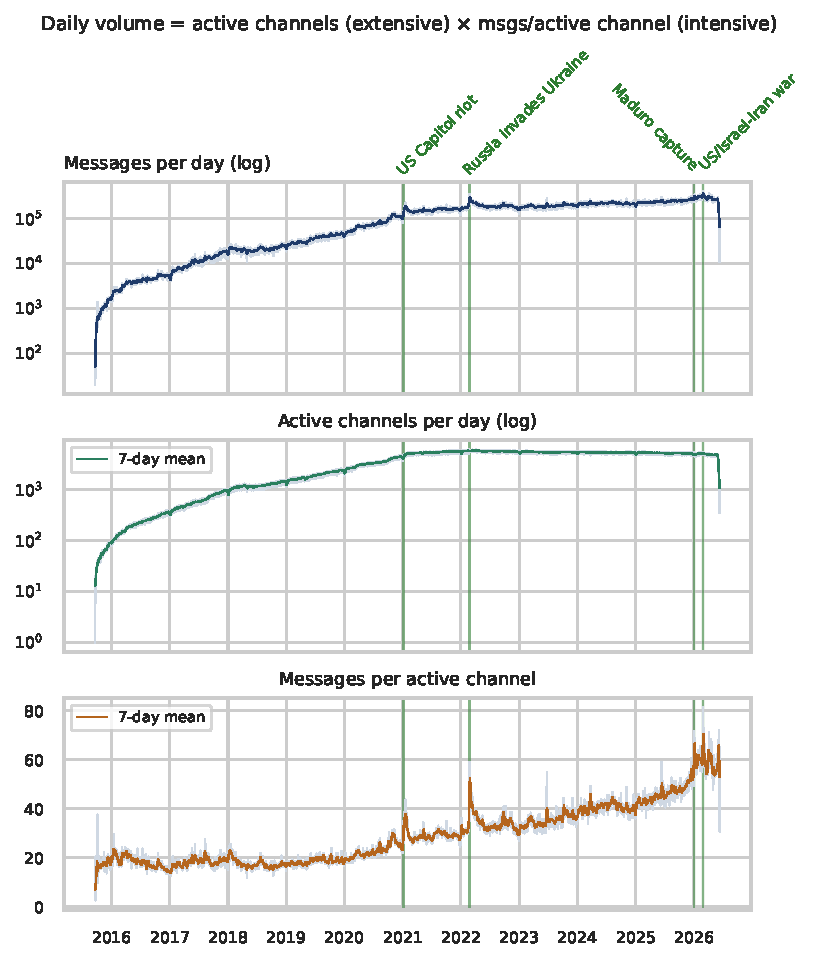
\includegraphics[width=\textwidth]{figures/res_daily_messages_normalised}
\caption[Daily message volume, decomposed.]{Daily message volume decomposed into extensive and intensive margins (Sep 2015 -- Jun 2026, $7$-day means; dashed lines mark external events). Top: total messages per day (log). Middle: number of channels active each day (log), the extensive margin. Bottom: mean messages per active channel each day, the intensive margin. The headline rise is almost entirely extensive (more channels active, saturating around 2021 as sampled channels enter the corpus); per-active-channel volume is far flatter, with only a modest recent rise and short event-driven spikes.}
\label{fig:res-daily-messages}
\end{figure}

\begin{figure}[htbp]
\centering
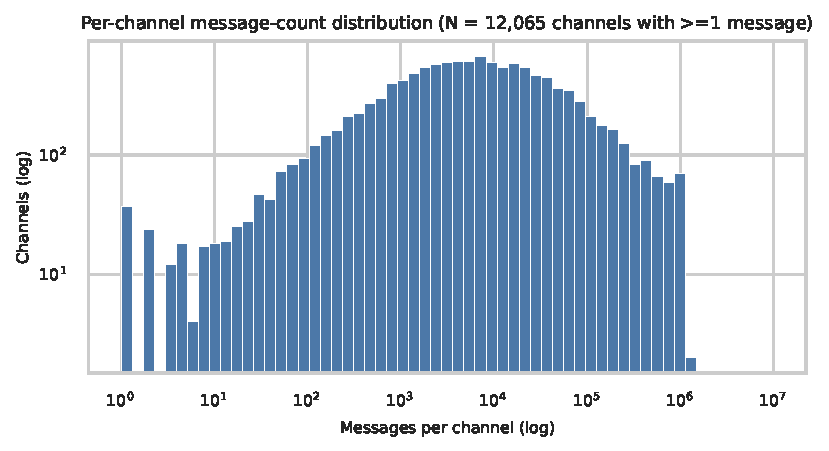
\includegraphics[width=\textwidth]{figures/res_channel_message_dist}
\caption[Per-channel message-count distribution.]{Distribution of per-channel lifetime message counts (log-binned, log--log axes). The distribution is unimodal: most of the $12{,}065$ crawled channels hold between $10^3$ and $10^4$ messages, with a long upper tail reaching past $10^6$. Depth spans several orders of magnitude, so the median channel is far shallower than the deepest, and a minority of very deep channels carries the corpus, which is why per-channel depth, not channel count, is the right scale on which to read this dataset.}
\label{fig:res-channel-depth}
\end{figure}

\paragraph{Posting follows a clear diurnal and weekly rhythm.}
The timing of posting characterises the active population as much as its size does. Figure~\ref{fig:res-activity-heatmap} aggregates message timestamps over the last twelve months into an hour-of-day by day-of-week grid (UTC), so it reflects the corpus's current posting rhythm rather than its full history. Activity follows a single broad daytime cycle: it bottoms out overnight ($00$--$03$\,UTC) and peaks in the afternoon and early evening, with the busiest hours between $14$ and $18$\,UTC and the single busiest cell on Wednesday around $18$\,UTC. The $08$--$20$\,UTC window carries about $70\%$ of all messages, and the busiest hour runs over three times the volume of the quietest. The weekly pattern is milder: weekend days sit about $13\%$ below the weekday average rather than collapsing, consistent with a feed of news and broadcast channels that post across the whole week rather than office-hours communication. Because timestamps are in UTC and channels span many time zones, this tight single-peak daytime concentration points to a corpus centred on European and Eurasian time zones, matching the Russian-dominant language mix reported in Section~\ref{sec:res-content}.

\begin{figure}[htbp]
\centering
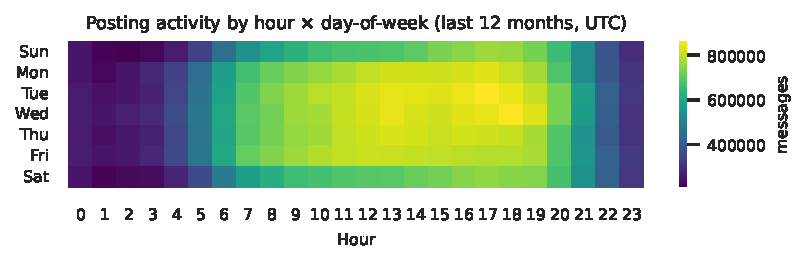
\includegraphics[width=\textwidth]{figures/res_activity_heatmap}
\caption[Posting-activity heatmap.]{Posting activity by hour of day and day of week over the last twelve months (UTC). Activity follows a single daytime cycle peaking in the afternoon and early evening ($14$--$18$\,UTC) and bottoming out overnight; weekend days are modestly quieter than weekdays.}
\label{fig:res-activity-heatmap}
\end{figure}

%======================================================================
\section{Reading the Forward Graph}
\label{sec:res-network}
%======================================================================

The forward references recorded in the corpus reconstruct a directed forward graph. A large fraction of the forwards in that graph are not editorial reposts but automatic copies: when a channel has a linked discussion group, Telegram mirrors each broadcast post into that group as a forward so comments can attach to it. This section removes those copies first, then reports every forward-graph statistic on the cleaned (\emph{editorial}) graph, because the correction has to be in place before any forward-based figure used elsewhere can be trusted.

\paragraph{Auto-mirror copies inflate the forward ratio.}
These auto-mirror copies are forwards in the data but carry no editorial meaning, and they make the raw forward ratio misleading. Of all messages, $18.3\%$ are flagged as forwarded (the raw forward ratio), but $34.0\%$ of those flagged forwards are auto-mirror duplicates; removing them yields an \emph{editorial} forward ratio of $12.1\%$, a $-6.2$ percentage-point correction (Table~\ref{tab:res-fwd-ratio}). Any ``what fraction of Telegram is reposted content'' figure taken from the raw flag therefore overstates editorial reposting by about a third. Every forward-graph result below is computed on the editorial graph, with auto-mirror edges removed.

\begin{table}[htbp]
\centering
\caption[Auto-mirror-corrected forward ratio.]{The forward ratio before and after removing auto-mirror duplicates (a channel's posts copied into its own linked group). Editorial reposting is $12.1\%$ of messages, not the $18.3\%$ the raw flag suggests.}
\label{tab:res-fwd-ratio}
\small
\begin{tabular}{@{}lr@{}}
\toprule
\textbf{Metric} & \textbf{Value} \\
\midrule
Raw forward ratio (\texttt{is\_forwarded} / all messages) & $18.3\%$ \\
Auto-mirror duplicates as share of all flagged forwards   & $34.0\%$ \\
Editorial forward ratio (auto-mirror removed)             & $12.1\%$ \\
Correction                                                & $-6.2$\,pt \\
\bottomrule
\end{tabular}
\end{table}

Removing auto-mirror does more than move the ratio: it changes what the graph looks like. The mirror edges are few but heavy, just $3{,}752$ \mbox{(parent~$\rightarrow$~own-group)} edges, barely a tenth of a percent of the graph, carry about $36\%$ of all forward weight, so on the full graph the largest forwarding community and the top hubs are discussion groups, an artefact of those edges; on the editorial graph ($401{,}928$ nodes, $2.9$\,M edges) the top communities and hubs are broadcast channels, as they should be. The editorial graph is a single giant weakly connected component, and reciprocal forwarding is negligible (the largest strongly connected component is $1.6\%$ of nodes), so forwarding is overwhelmingly one-directional: a small set of source channels feed a large set of repackagers.

\paragraph{Repost networks, not virality.}
Telegram rewrites forward metadata to point at the original sender along the whole chain, so recursive walks over \texttt{fwd\_\allowbreak from\_\allowbreak channel\_\allowbreak id} structurally bottom out at depth~one. The most-forwarded source message in the corpus accumulated $1{,}570$ in-corpus forwards from only four distinct channels, all at depth~one. ``Most-forwarded'' rankings therefore surface dense repost clusters, not viral multi-hop diffusion.

\subsection{The Reference Frontier}
\label{sec:res-frontier}

The corpus records a large frontier of channels it has seen referenced but never crawled. Part of the frontier is permanently out of reach. Of $2.28$\,M hyperlinked \texttt{t.me} references, only about $52\%$ are plain queue-able public handles; roughly $14\%$ are invite-only \texttt{+hash} or web-preview links that our scraper's capture group can never resolve, and a further $24.5\%$ are deep links that point at a message inside an already-queued channel (Figure~\ref{fig:res-frontier}). The invite-only share is a hard structural ceiling rather than a backlog. The unreachable set features clusters by theme (Russian-military and geopolitics discussion, German far-right, Iranian news) and includes the uncrawled discussion groups of major channels such as Kinopoisk, Kommersant, and Khamenei-affiliated news.

\begin{figure}[htbp]
\centering
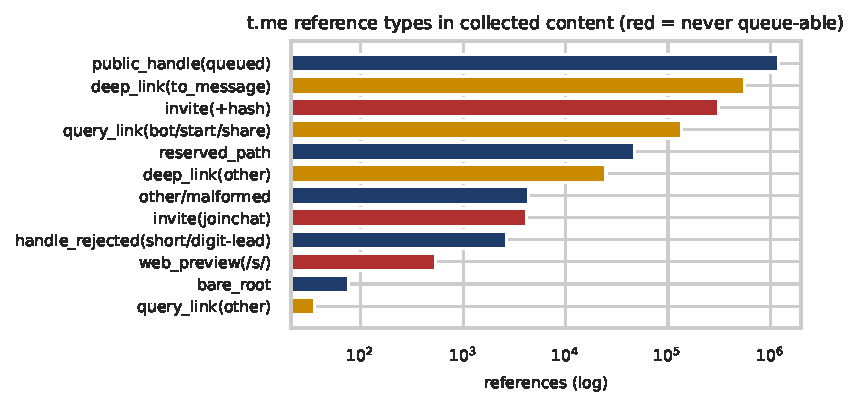
\includegraphics[width=\textwidth]{figures/res_frontier_link_types}
\caption[Frontier link-type breakdown.]{Breakdown of cited \texttt{t.me} references by link type. About half are queue-able public handles; invite-only and web-preview links (roughly $14\%$) are a hard structural ceiling, and deep links (about $24.5\%$) point into already-queued channels.}
\label{fig:res-frontier}
\end{figure}

%======================================================================
\section{Combined Capability Layers}
\label{sec:res-layers}
%======================================================================

This section presents the capabilities that justify the dataset, each traced to the collection mechanism that produced it. The first three subsections cover comments, edits, and deletions; the edit and deletion layers are collected by no prior general-purpose Telegram corpus, and the comment layer only by the concurrent TeraGram~\cite{teragram2026} (and there as a single static snapshot, without the edit and deletion history we pair with it); the fourth covers per-platform restriction, present but unexposed inside serialized message objects in prior corpora and surfaced and analysed here at scale; the fifth gathers in the supporting content surface; the sixth records what we deliberately did \emph{not} find.

\subsection{Comments and Discussion}
\label{sec:res-comments}

A comment is not a first-class object on Telegram. When a broadcast channel turns comments on, the platform attaches a linked discussion group and mirrors every post into it as a byte-identical copy that the channel itself posts (an auto-forward); the comment thread a reader sees is just the set of replies to that mirrored copy. The scraper collects this layer by following the parent's linked-group pointer, registering the group as a \texttt{linked\_group} child with a back-pointer to its parent, and scraping it inline within the same per-channel turn rather than as a separate queue entry (Section~\ref{sec:scraping-cycle}). That design is what turns ``comments'' from an unreachable interface affordance into stored, queryable rows, and it is the mechanism behind the single largest additive layer in Table~\ref{tab:res-scalars}: the $333.2$\,M-message discussion side, which among general-purpose corpora only the concurrent TeraGram~\cite{teragram2026} collects by design.

Comments are identified structurally rather than from the raw \texttt{is\_comment} flag, which the scraper hard-codes to \texttt{false} on every row at collection time. The flag is populated only afterward, by a backfill pass (\texttt{tools/set\_is\_comment.py}) that classifies each discussion-group message by how it attaches to the post stream:

\begin{itemize}
\item An \emph{auto-mirror} is the thread head: the byte-identical copy of a parent post that the channel itself auto-forwards into the group, recognised as channel-authored by \texttt{author\_id} equal to the parent.
\item A \emph{comment} is a reply that anchors on an auto-mirror, either directly (its \texttt{reply\_\allowbreak to\_\allowbreak msg\_\allowbreak id} targets the mirror) or through its thread root (\texttt{reply\_\allowbreak to\_\allowbreak top\_\allowbreak id}) on a nested reply. These are the only rows the flag marks \texttt{true}.
\item \emph{Everything else} stays \texttt{false}: the auto-mirrors themselves (channel copies, not reader replies), free in-group chat (top-level messages with no reply pointer), and replies that answer another member rather than a post.
\end{itemize}

Because the rule keys on the auto-mirror, a comment whose thread-head mirror was never captured (deleted, or outside the crawled range) is missed, so the backfilled flag is a \emph{lower bound} on comments, the counterpart to the reply-pointer count introduced next, which over-states them.

On that structural definition, comments are a plurality of the corpus: $202.5$\,M messages ($42.6\%$ of all messages) carry a reply pointer, and $198.2$\,M of those ($97.9\%$) sit inside a crawled linked discussion group. The comment layer alone is therefore larger than the entire broadcast side ($141.8$\,M). This is a direct consequence of the depth-first design of Section~\ref{sec:res-corpus}: the deepest channels in the corpus are overwhelmingly discussion groups, so sampling fewer channels far more thoroughly disproportionately fills in the comment side. These reply-bearing messages are the layer's raw extent, but they are an \emph{upper bound} on genuine comments-on-posts, for the reason the next correction makes precise.

A reply pointer only records that a message answers some earlier message; it does not record that the earlier message was a broadcast post. Genuine comments-on-posts anchor, directly or transitively, on the mirrored duplicate of a parent post, and that duplicate is byte-identical to the original in $99.8\%$ of matched cases ($47{,}285$ of $47{,}379$), so anchoring can be checked directly rather than assumed. (These mirrored duplicates are exactly the auto-mirror forwards whose contamination of the forward graph Section~\ref{sec:res-network} removes: the thread head a comment replies to is the same edge that inflates the raw forward ratio.) Checking anchoring per group reveals a sharply bimodal population (Figure~\ref{fig:res-anchoring}): the median discussion group anchors $79.4\%$ of its replies on a post, behaving as a true comment section, while a handful of very high-volume chat-style groups reply mostly to one another and drag the reply-weighted pooled anchoring rate down to $58.2\%$. The reply-pointer count therefore over-states comments-on-posts by roughly $42\%$ corpus-wide (about $21\%$ for the median group), and the de-biased comments-on-posts estimate is near $58\%$ of the $198.2$\,M reply-bearing total. The separation of a post-anchored comment section from free in-group chat is itself a finding the discussion-group side cannot be read without. Table~\ref{tab:res-comment-decomp} sets out the resulting decomposition of the whole discussion side, separating the mirrored posts themselves, the comment threads anchored on them, and the in-group messages that carry no mirrored-post reference.

\begin{figure}[htbp]
\centering
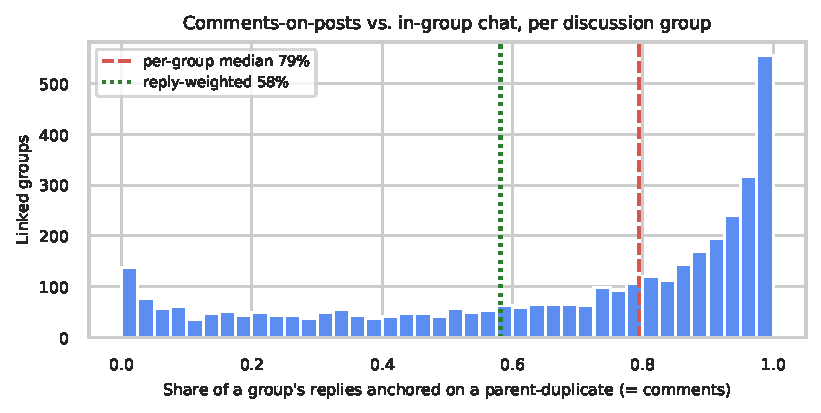
\includegraphics[width=\textwidth]{figures/res_anchoring_rate_dist}
\caption[Comment anchoring-rate distribution.]{Per-group anchoring rate: the share of a discussion group's replies that attach to a mirrored broadcast post rather than to other in-group chat. The distribution is bimodal. Most groups behave as true comment sections (median $79.4\%$), while a few high-volume chat-style groups anchor little and pull the reply-weighted pooled rate down to $58.2\%$, which is why the raw reply-pointer count over-states comments-on-posts.}
\label{fig:res-anchoring}
\end{figure}

\begin{table}[htbp]
\centering
\caption[Decomposition of the linked-group discussion side.]{Decomposition of the $333.2$\,M-message linked-group discussion side into mutually exclusive populations. A member manually forwarding a parent post into the group looks identical on the \texttt{fwd\_from} fields but is sent by a user, so the $0.15$\,M such forwards ($0.5\%$ of matching \texttt{fwd\_from} rows) are counted as standalone messages, not mirrors. \emph{Comments on a mirror} are the replies that anchor, directly or transitively, on a mirrored post, that is, the comment threads of Figure~\ref{fig:res-anchoring}; the next row holds reply-bearing messages that anchor on something else (in-group conversation), and the last holds non-reply group messages. The final two rows together ($188.5$\,M) are the messages with no mirrored-post reference.}
\label{tab:res-comment-decomp}
\small
\setlength{\tabcolsep}{6pt}
\begin{tabular}{@{}lrr@{}}
\toprule
\textbf{Population} & \textbf{Messages} & \textbf{Share} \\
\midrule
Mirrored posts (auto-forward thread heads)          & $29.4$\,M  & $8.8\%$  \\
Comments on a mirror (anchored, incl.\ the thread)  & $115.2$\,M & $34.6\%$ \\
In-group messages not anchored to a mirror          & $82.9$\,M  & $24.9\%$ \\
Standalone group messages (no reply, no mirror)     & $105.6$\,M & $31.7\%$ \\
\midrule
Linked-group discussion side (total)                & $333.2$\,M & $100\%$  \\
\bottomrule
\end{tabular}
\end{table}

The broadcast side carries a complementary signal the discussion side cannot: whether comments were enabled for an individual post. Telegram attaches a replies object (stored as \texttt{replies\_count}, Table~\ref{tab:messages}) to a post only when comments are on for it, so on a broadcast that owns a discussion group, \texttt{replies\_count} being \texttt{NULL} marks comments disabled for that post, $0$ marks enabled-but-empty, and $>0$ marks enabled-with-comments. Across the $67.2$\,M non-service posts on channels that own a discussion group, $46.4\%$ are disabled, $36.8\%$ are enabled but drew no comment, and only $16.8\%$ actually carry comments (Table~\ref{tab:res-comment-toggle}). The decomposition separates a genuinely disabled post from one that was open but ignored, a distinction invisible from the group side where both look like a post with no thread. The toggle is also exercised \emph{within} channels rather than set once: many broadcasters carry both enabled and disabled posts (the interior mass of Figure~\ref{fig:res-comment-toggle}) instead of sitting at all-off or all-on. A capture cross-check corroborates the reading: posts marked enabled carry a matching mirrored duplicate in the linked group $61.4\%$ of the time against only $28.9\%$ for disabled posts, the expected direction, with the residual gap attributable to imperfect chat capture rather than to noise in the signal. What the field cannot show is why or when a post's comments were toggled, because only the latest \texttt{replies\_count} snapshot is stored, with no history.

\begin{table}[htbp]
\centering
\caption[Per-post comment toggle.]{Per-post comment state on the $67.2$\,M non-service broadcast posts belonging to channels that own a discussion group, read from \texttt{replies\_count}. Most posts have comments disabled or enabled-but-empty; only about one in six actually draws a comment. Because the state is read per post, it captures within-channel toggling that the discussion-group side cannot see.}
\label{tab:res-comment-toggle}
\small
\setlength{\tabcolsep}{6pt}
\begin{tabular}{@{}lrr@{}}
\toprule
\textbf{Per-post state} & \textbf{Posts} & \textbf{Share} \\
\midrule
Comments disabled (\texttt{replies\_count} NULL) & $31.2$\,M & $46.4\%$ \\
Enabled, no comments ($=0$)                       & $24.7$\,M & $36.8\%$ \\
Enabled, with comments ($>0$)                     & $11.3$\,M & $16.8\%$ \\
\bottomrule
\end{tabular}
\end{table}

\begin{figure}[htbp]
\centering
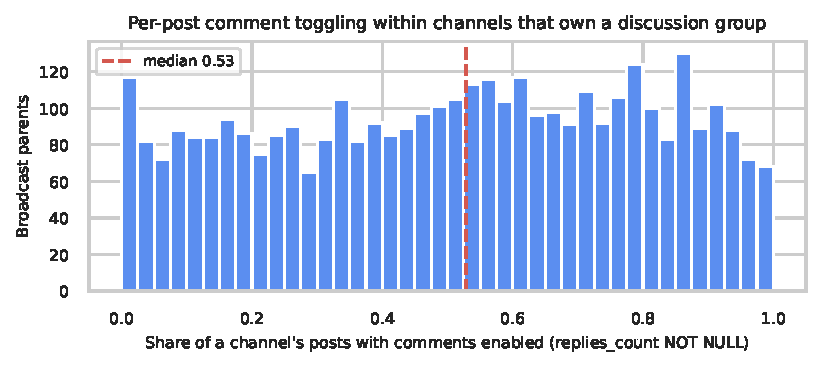
\includegraphics[width=\textwidth]{figures/res_comment_post_toggle}
\caption[Per-post comment toggling within channels.]{Distribution of broadcast channels by the fraction of their posts that have comments enabled. The interior mass shows that toggling is exercised per post within a channel rather than set once; the spikes at $0$ and $1$ are channels that run a single all-off or all-on policy.}
\label{fig:res-comment-toggle}
\end{figure}

Thread shape is best shown on one worked example. The Cycling Market channel and its linked chat hold $391$\,K broadcast posts against $999$\,K discussion messages, a commentariat roughly $2.6\times$ the size of the broadcast stream. Reconstructing reply trees over the chat gives the depth distribution of Figure~\ref{fig:res-thread-depth}: most comments are depth-one replies directly to the post, with a long tail of deeper back-and-forth. The commentariat is heavily concentrated, the two most active accounts alone contributing $18.4\%$ and $17.5\%$ of all human comments, and returning commenters outnumber first-time ones in every month after the section's launch. These thread-structure figures illustrate one active comment section rather than the whole corpus, but they show the granularity the layer supports (per-account, per-thread, and longitudinal), and the moderation behaviour of this layer (comments are deleted about four times as often as posts) is taken up in Section~\ref{sec:res-deletion}.

\begin{figure}[htbp]
\centering
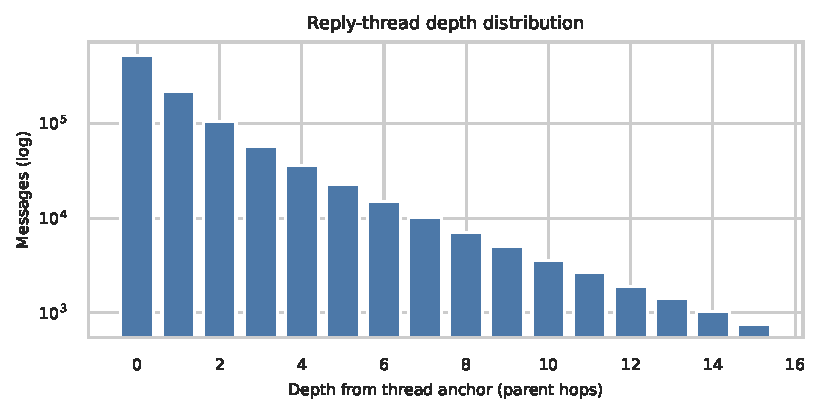
\includegraphics[width=\textwidth]{figures/res_thread_depth_dist}
\caption[Comment thread depth.]{Reply-tree depth distribution for one worked comment section (Cycling Market). Most comments sit at depth one, direct replies to the post; a long tail of deeper threads reflects back-and-forth between commenters.}
\label{fig:res-thread-depth}
\end{figure}

\subsection{Edits: What They Actually Do}
\label{sec:res-edits}

The before/after text of edited messages is a capability no flag-only corpus has, and it overturns the natural proxy for editing. Telegram's permanent \texttt{edit\_date} flag is set on roughly one third of all messages, but it is not a human-edit signal: about $20\%$ of flagged edits land within ten seconds of posting, and roughly three quarters of those are Telegram auto-finalising media albums and link previews rather than a person changing anything (Figure~\ref{fig:res-edit-auto}). Text-only edits, by contrast, skew late.

The diffable archive, the $36{,}016$ edits for which the scraper caught both versions, settles what editing actually does. Of these, $93\%$ leave the message text byte-identical, with the change confined to media, markup, or message entities; the $7\%$ that do rewrite text come to $2{,}356$ before/after pairs, which Claude Sonnet~4.6~\cite{claudesonnet2026} labels against a fixed taxonomy; grouping those labels splits the set $62\%$ substantive editorial against $38\%$ non-substantive. For each pair the model is given the archived before-text and the current after-text and asked to assign exactly one primary label, the \emph{dominant} kind of change, from a fixed nine-type taxonomy (cosmetic, mechanical-counter, factual correction, addition, removal, tone rewrite, compliance annotation, multi, and other) and to add a short free-text note naming the concrete change; the prompt instructs it to judge the change rather than the language, since the corpus is multilingual. Two of the nine types (cosmetic fixes and auto-updating tallies such as vote or view counts) are defined as non-substantive, and that boundary is what draws the $62/38$ line. The full labelling prompt is reproduced in Appendix~\ref{app:edit-prompt}. The single largest type is cosmetic typo, spacing, and markup fixes ($36\%$), followed by additions ($23\%$) and removals ($13\%$), with substantive rewrites, factual corrections, and entity swaps making up the remainder (Figure~\ref{fig:res-edit-taxonomy}). Two further properties sharpen what an edit is for. First, editing is essentially \emph{valence-neutral}: scored with the \texttt{textdetox} XLM-R toxicity classifier~\cite{dementieva2024}, $97\%$ of edits move a message's toxicity by at most $0.05$ on a $0$--$1$ scale, so editing is not systematic de/toxification or sentiment-laundering. Second, what substantive edits churn is \emph{facts}, not tone: a number changes in $39\%$ of them, and under a multilingual named-entity tagger~\cite{tedeschi2021} the most-edited entity types are miscellaneous ($24\%$), locations ($12.6\%$), persons ($11.7\%$), and organisations ($10.2\%$), with additions and deletions roughly balanced per type, that is, substitution rather than net accretion. Editing is also concentrated and skews toward large official channels. The contribution here is a measured replacement for a widely misused flag: the raw flag over-counts human editing by roughly an order of magnitude, and the before/after archive supplies the corrected picture, down to what the edits actually rewrite. The edit-detection mechanism is described in Section~\ref{sec:combined-pass}.

\begin{figure}[htbp]
\centering
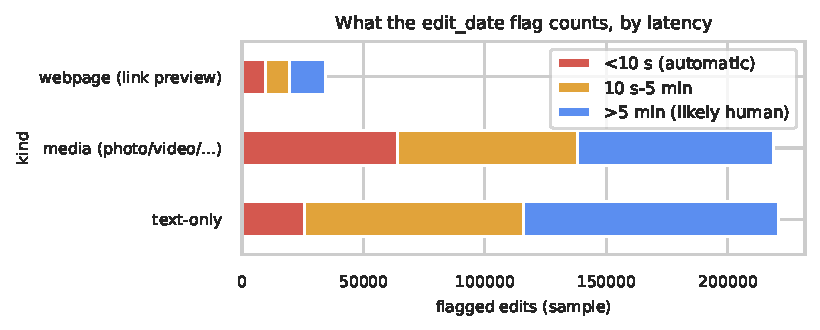
\includegraphics[width=\textwidth]{figures/res_edit_automatic_vs_genuine}
\caption[Automatic vs.\ genuine edits.]{Edits by content kind and time-to-edit. The early spike is dominated by media and link-preview finalisation (automatic), not human editing; text edits arrive later. This is why \texttt{edit\_date} over-counts genuine editing.}
\label{fig:res-edit-auto}
\end{figure}

\begin{figure}[htbp]
\centering
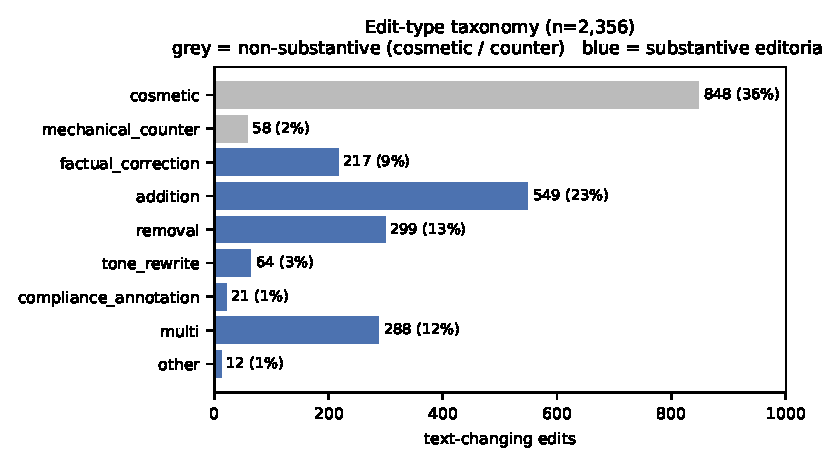
\includegraphics[width=\textwidth]{figures/res_edit_taxonomy}
\caption[Edit-type taxonomy.]{Distribution of the $2{,}356$ text-changing edits across a fixed type taxonomy. A clear majority ($62\%$) are substantive editorial changes (additions, removals, factual corrections, entity swaps) rather than non-substantive ones ($38\%$), of which cosmetic typo and markup fixes are the single largest type at $36\%$.}
\label{fig:res-edit-taxonomy}
\end{figure}

\subsection{Deletion: Thread Purges and Group-Internal Moderation}
\label{sec:res-deletion}

Deletion tracking lets us ask who deletes and whether deletion propagates. Comments are deleted substantially more often than posts: the comment deletion rate is $0.78\%$ against $0.18\%$ for broadcast posts and $0.11\%$ for auto-forward heads (Table~\ref{tab:res-deletion-rates}, Figure~\ref{fig:res-deletion-rates}). Heads are deleted far less than posts, so post deletion is not, in general, sweeping the whole thread away through the mirror copy.

Where deleted comments sit tells a more specific story. Of all deleted comments, $61\%$ sit under a deleted post-thread head, that is, the parent post was itself deleted, so the dominant pattern is thread-level removal: when a post goes, the comments under it go with it (Figure~\ref{fig:res-deletion-root}). The remaining $\sim39\%$ is group-internal: comments removed off a still-alive root ($15\%$), off a deleted native group message ($18\%$), or off a deleted forwarded-in post ($6\%$), reflecting independent moderation and self-deletion inside the group. The capability separates two phenomena the literature tends to conflate: thread-purge deletion driven from the broadcast side, and in-group moderation that the post author never sees.

This split is a property of the collected deleted set, not of deletion on Telegram in general: deletions are detected only on revisit and within a short detection window, so the $2.42$\,M detected deletions are a partial, detection-time sample, and the precise balance between thread-purge and group-internal removal should be read with that sampling in mind. The content of deleted messages is also distinctive. Deleted messages are shorter than surviving ones (median $74$ against $88$ characters) and markedly link-poorer ($4.9\%$ carry a URL against $13.4\%$), and their most over-represented content is spam-token strings and Telegram terms-of-service removal templates rather than any political topic. Deleted content is also more toxic than what survives: against a server-shuffled surviving control, deleted messages score $1.62\times$ higher on the \texttt{textdetox} XLM-R toxicity classifier (mean $0.206$ against $0.128$). That lift is not uniform across the two removal regimes, which target different content: independent in-group moderation, where the parent post survives, removes markedly more-toxic content than a blanket thread-purge that sweeps a whole conversation regardless of content (mean toxicity $0.247$ against $0.187$; Figure~\ref{fig:res-moderation-purge}). Editorial choice targets toxic comments; a thread-purge does not.

Deletion is also concentrated in time: rather than removing content as a steady trickle, a few large discussion groups shed between $100{,}000$ and $320{,}000$ messages in a single day. These spikes are not one phenomenon. Telegram numbers a channel's messages sequentially, so the positions of the deleted ids reveal how a purge was carried out: one long run of consecutive ids means a contiguous block was removed at once, whereas many short runs scattered among surviving ids mean messages were taken out individually. Read this way, the $115$ channels that hold $98\%$ of all purge volume split into three regimes:

\begin{itemize}
\item \textbf{Block-window purges} ($47.3\%$ of the volume): one long contiguous interval, eg. a group clearing its \emph{older} content over a date window while the rest of the channel lives on.
\item \textbf{Scattered moderation} ($35.1\%$): many short intervals interleaved with survivors, eg. a group removing individual comments while the rest of the thread survives.
\item \textbf{Whole-channel wipes} ($17.6\%$): almost the entire channel ($\geq 95\%$) gone in a single detection window.
\end{itemize}

The one-day framing is itself partly an artefact of detection. Because deletions are noticed only on revisit, $87$ of the $115$ channels carry a single detection timestamp: weeks of removals collapse onto the one day the scraper next looked, so a ``purge day'' is a detection event, not necessarily one atomic deletion. The regimes also differ in what they remove. The whole-channel wipes are coherent dead communities taken out wholesale (state-media discussion, anti-vaccine conspiracy, crypto-scam spam), the signature of a channel being taken down or abandoned. The block-window purges instead clear ordinary discussion groups' older content, including 2026 Iran--Israel war chatter, the same event whose two official cohorts the war showcase reads directly for audience toxicity (Section~\ref{sec:res-war}). The deletion-detection mechanism is described in Section~\ref{sec:combined-pass}.

\begin{table}[htbp]
\centering
\caption[Deletion rates by role.]{Detected deletion rate by message role. Comments are deleted about four times as often as broadcast posts; auto-forward heads least of all.}
\label{tab:res-deletion-rates}
\small
\begin{tabular}{@{}lrr@{}}
\toprule
\textbf{Role} & \textbf{Deleted / total} & \textbf{Rate} \\
\midrule
Comment            & $1{,}537{,}202 / 198.2$\,M & $0.78\%$ \\
Broadcast post     & $259{,}617 / 141.8$\,M     & $0.18\%$ \\
Auto-forward head  & $32{,}328 / 29.4$\,M       & $0.11\%$ \\
\bottomrule
\end{tabular}
\end{table}

\begin{figure}[htbp]
\centering
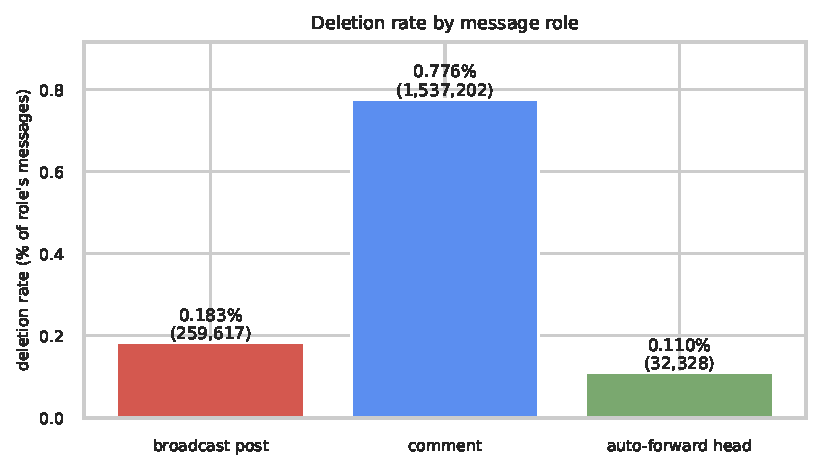
\includegraphics[width=\textwidth]{figures/res_deletion_rates_by_role}
\caption[Deletion rates by role.]{Detected deletion rate by message role. Comments delete more readily than posts; auto-forward heads least, so post deletion does not propagate into the group through the mirror copy at scale.}
\label{fig:res-deletion-rates}
\end{figure}

\begin{figure}[htbp]
\centering
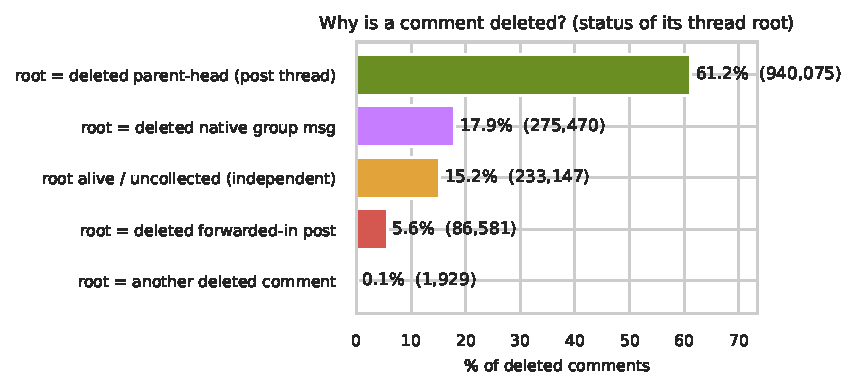
\includegraphics[width=\textwidth]{figures/res_deleted_comment_root_status}
\caption[Deleted-comment root status.]{Where deleted comments sit. A majority ($61\%$) are under a deleted post-thread head (thread-level purge); the remainder are group-internal moderation or self-deletion off still-alive or independently deleted roots.}
\label{fig:res-deletion-root}
\end{figure}

\begin{figure}[htbp]
\centering
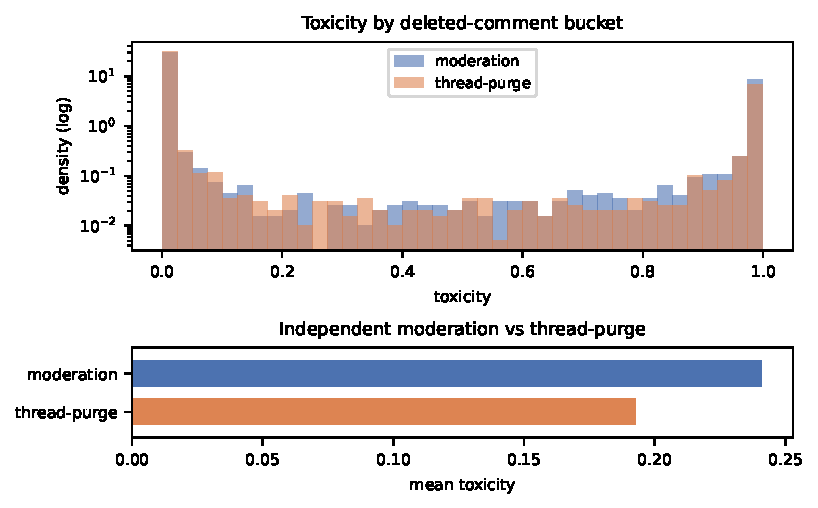
\includegraphics[width=\textwidth]{figures/res_moderation_vs_purge}
\caption[Moderation versus thread-purge toxicity.]{Toxicity of deleted comments split by removal regime. Top: the full toxicity distribution per regime. Bottom: mean toxicity per regime. Independent in-group moderation, where the parent post survives, removes more-toxic content (mean $0.247$) than a blanket thread-purge that removes a whole conversation regardless of content (mean $0.187$), a $1.32\times$ gap. Toxicity scored with the \texttt{textdetox} XLM-R classifier.}
\label{fig:res-moderation-purge}
\end{figure}

\subsection{Restriction and High-Harm Content at Scale}
\label{sec:res-restriction}

The per-platform \texttt{restriction\_reason} flag is a content signal that prior corpora retained only inside serialized message objects and never exposed or analysed; we surface it as a first-class field and study it at scale, a substantial net-new content signal in its own right. $18.7$\,M messages carry at least one restriction flag, indicating content hidden on a specific platform rather than removed (Figures~\ref{fig:res-restriction} and~\ref{fig:res-restriction-platform}, Table~\ref{tab:res-restriction}). The drivers are platform policy, not state censorship: the flags are iOS-heavy, and the largest single content reason is \texttt{porn} ($7.6$\,M flag instances), almost entirely on iOS, reflecting Apple's App~Store rules. A separate and far smaller phenomenon is whole-post obscuring, where Telegram replaces a post's entire content with a service notice that the channel cannot be displayed because it violated the platform's terms of service ($123$\,K such messages in our corpus). This is the form prior work already surfaced: TGDataset reported these obscuring service messages as per-reason counts (its Table~4~\cite{lamorgia2025}). It is also more terminal than per-platform restriction: $13.1\%$ of obscured posts are also deleted, against only $0.8\%$ of restriction-flagged posts. The genuinely net-new signal here is instead the per-platform \texttt{restriction\_reason} field, which prior corpora left untouched; because it is stored as a first-class column (Table~\ref{tab:messages}), these slices are directly queryable.

The same reading holds across language communities once raw counts are normalised (Figures~\ref{fig:res-restriction-lang} and~\ref{fig:res-restriction-lang-rate}). Raw flag instances track representation, English and Russian dominate because they carry the most messages, but the restriction \emph{rate} (flags per $1{,}000$ messages) flips the picture: Russian is among the least restriction-prone communities ($2.3\%$ of messages flagged), while the most restriction-prone are smaller ones, Chinese ($53.8\%$), Polish ($53.1\%$), and Arabic ($49.9\%$), each driven by a single app-store category. Across every language the reasons that survive normalisation are app-store policy categories (\texttt{porn}, \texttt{androidterms}, \texttt{appleterms}, \texttt{appleviolence}), not the Telegram-level \texttt{terms} reason; restriction-proneness varies by community, but the mechanism is App~Store and Play~Store enforcement, not language-specific state censorship. These reason categories also co-occur within the same channels (Figure~\ref{fig:res-restriction-cooccurrence}): a channel hidden under one store category is typically hidden under others, as expected when a single store policy suppresses the same content under several reason codes.

The layer also supports high-harm content slicing, and the behaviour differs sharply by content type. A crypto pump-and-dump cluster deletes at roughly $5.6\times$ the corpus baseline and forwards less, a self-scrubbing pattern, while an extremist cluster barely deletes but forwards more and is comment-heavy, an unrepentant and discussion-driven one. These are rates within our corpus, not absolute prevalence claims.

\begin{table}[htbp]
\centering
\caption[Restriction reasons by flag instances.]{Top per-platform restriction reasons. A message can be flagged on several platforms, so counts are flag instances; the flags are dominated by app-store policy categories, not state moderation.}
\label{tab:res-restriction}
\small
\setlength{\tabcolsep}{6pt}
\begin{tabular}{@{}lrr@{}}
\toprule
\textbf{Reason} & \textbf{Flag instances} & \textbf{Channels} \\
\midrule
\texttt{androidterms}  & $10.57$\,M & $2{,}740$ \\
\texttt{porn}          & $7.63$\,M  & $2{,}402$ \\
\texttt{appleviolence} & $5.05$\,M  & $2{,}194$ \\
\texttt{appleterms}    & $4.27$\,M  & $2{,}402$ \\
\texttt{copyright}     & $0.99$\,M  & $2{,}422$ \\
\texttt{terms}         & $0.19$\,M  & $1{,}815$ \\
\bottomrule
\end{tabular}
\end{table}

\begin{figure}[htbp]
\centering
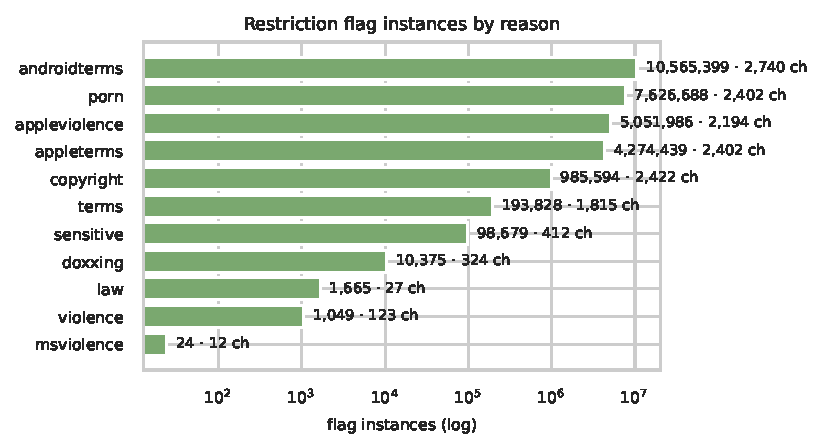
\includegraphics[width=\textwidth]{figures/res_restriction_reasons_by_reason}
\caption[Per-platform restriction by reason.]{Per-platform restriction flag instances grouped by reason, on a $\log_{10}$ scale (flag-instance and channel counts annotated). The flag is dominated by app-store policy categories such as \texttt{androidterms} and \texttt{porn}, indicating store-policy hiding rather than state censorship.}
\label{fig:res-restriction}
\end{figure}

\begin{figure}[htbp]
\centering
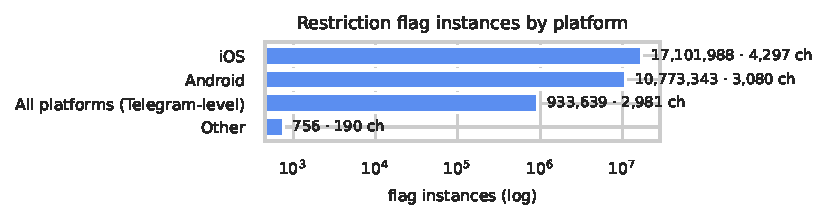
\includegraphics[width=\textwidth]{figures/res_restriction_reasons_by_platform}
\caption[Per-platform restriction by platform.]{The same restriction flag instances grouped by the platform on which the content is hidden, on a $\log_{10}$ scale. Restriction is iOS-heavy, with Android second and a smaller Telegram-level ``all platforms'' share; the opaque minor codes \texttt{VIRT1} and \texttt{ms} (under $10^3$ instances combined) are collapsed into a single \emph{Other} bucket.}
\label{fig:res-restriction-platform}
\end{figure}

\begin{figure}[htbp]
\centering
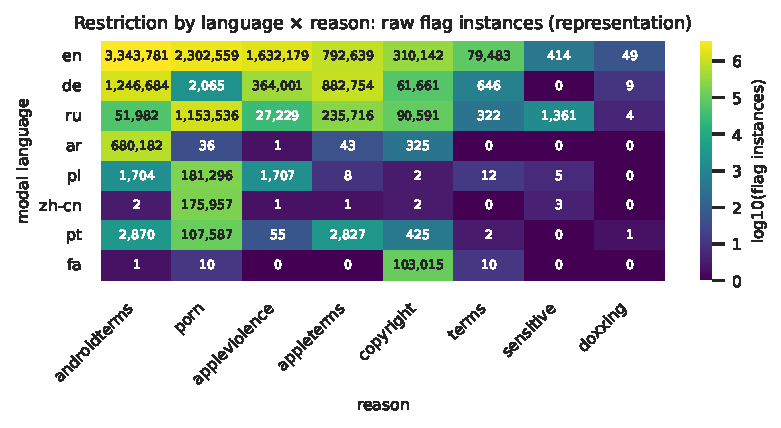
\includegraphics[width=\textwidth]{figures/res_restriction_lang_reason_raw}
\caption[Restriction by language and reason: raw flag instances.]{Restriction by language $\times$ reason, raw flag instances on a $\log_{10}$ colour scale. Raw counts track representation: English and Russian dominate because they carry the most messages, not because those communities are the most restriction-prone (see the normalised view, Figure~\ref{fig:res-restriction-lang-rate}).}
\label{fig:res-restriction-lang}
\end{figure}

\begin{figure}[htbp]
\centering
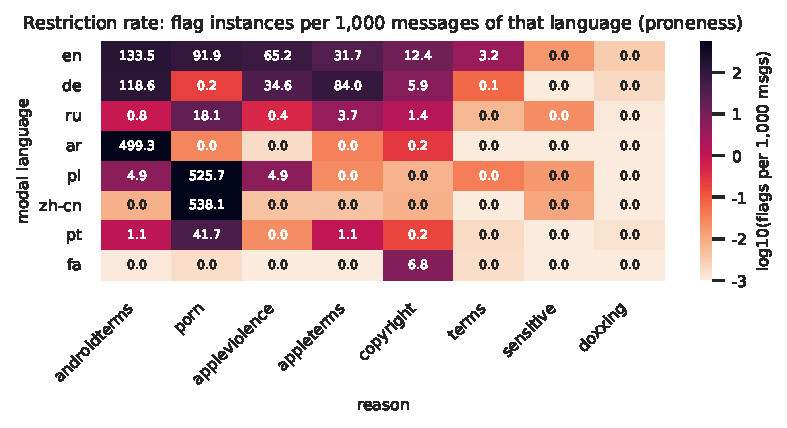
\includegraphics[width=\textwidth]{figures/res_restriction_lang_reason_rate}
\caption[Restriction by language and reason: normalised rate.]{Restriction rate, flag instances per $1{,}000$ messages in each language, on a $\log_{10}$ colour scale. Normalisation isolates restriction-proneness: the communities that survive it (Chinese, Polish, Arabic) are driven by app-store categories (\texttt{porn}, \texttt{androidterms}), not by the Telegram-level \texttt{terms} reason, which is negligible across all languages.}
\label{fig:res-restriction-lang-rate}
\end{figure}

\begin{figure}[htbp]
\centering
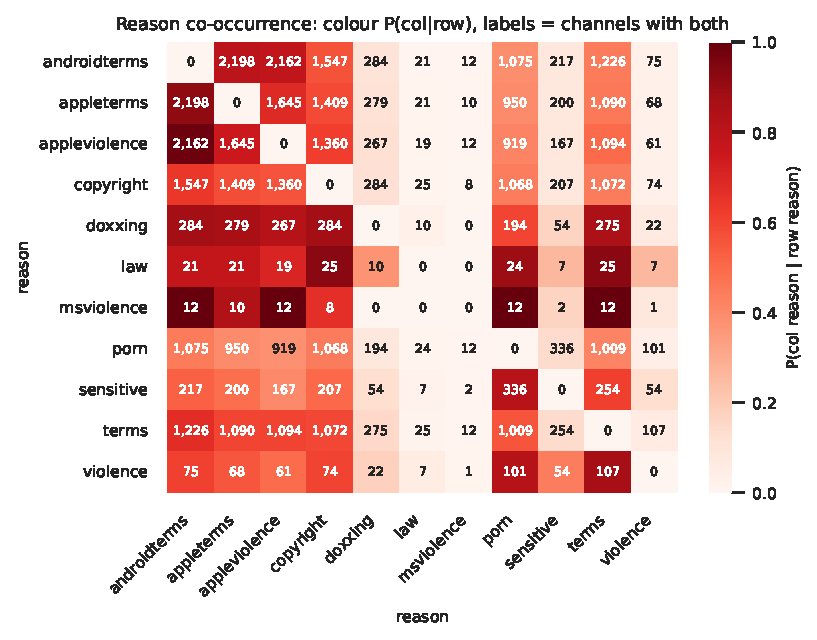
\includegraphics[width=\textwidth]{figures/res_restriction_cooccurrence}
\caption[Restriction reason co-occurrence.]{Co-occurrence of restriction reasons within a channel. Cell colour is the row-conditional share $P(\text{column reason}\mid\text{row reason})$ and the annotation is the number of channels carrying both reasons. The app-store policy categories tend to co-occur within the same channels, consistent with a single store policy hiding the same content under several reason codes rather than reason-specific moderation.}
\label{fig:res-restriction-cooccurrence}
\end{figure}

\subsection{The Content Surface: Engagement, Language, Polls, and Service Actions}
\label{sec:res-content}

The corpus is multilingual, dominated by Russian ($52\%$ of majority-language channels), then English ($18\%$), German ($9\%$), Ukrainian ($5\%$), and Farsi ($5\%$) (Figure~\ref{fig:res-language}); the English share matches TGDataset's $16\%$ almost exactly, while Russian is over-represented relative to it, a composition difference rather than a platform change. Topic shares from a BERTopic model~\cite{grootendorst2022} over the English-language channels are shown in Figure~\ref{fig:res-topics}, led by political news, then COVID and vaccine content, then religion. The language boundary is also a forwarding boundary: channels keep almost all of their forwards in-language (Farsi $99.7\%$, Russian $98.0\%$, German $95.7\%$, English $90.0\%$ of each language's outbound forwards stay same-language), and the dominant language of a linked discussion group matches its parent channel's in nearly every pair. The main exceptions are a modest English--German exchange (about $3$--$5\%$ of forwards each way) and a Russian--Ukrainian bilingual zone, where Ukrainian channels route roughly $15\%$ of their forwards to Russian-language sources and which accounts for almost all of the few group-to-parent language mismatches.

The structured reaction surface supports a genuine but correlational observation: in the most-negatively-reacted-to decile of channels the verified rate is roughly twice that of the most-positive decile ($7.1\%$ against $3.3\%$), and those channels are also several times larger by subscriber count, so the blue check tracks prominence and controversy rather than vetted safety (Figure~\ref{fig:res-verified}). The polls layer ($323$\,K polls) makes both turnout and vote-distribution shape analysable: turnout (voters per view) is recorded for almost every poll and runs at a median of $0.255$, while the $27{,}567$ polls that also store per-option tallies expose the full vote distribution (Figure~\ref{fig:res-polls}); Arabic and Farsi polls stand out as both larger and better attended (median turnout $0.35$ and about $2{,}500$ voters) than the Cyrillic majority (median turnout $0.24$, about $590$ voters). The service-action stream separately records pinning, chat-to-supergroup migrations, and gift and boost adoption (Figure~\ref{fig:res-service}). One language-cohort result deserves a forward pointer: the Farsi cohort is notably ban-resilient, with $99\%$ of channels active before Iran's 2018 Telegram ban~\cite{iranban2018} still active afterward and most still active in 2026. We develop it in the war showcase.

\begin{figure}[htbp]
\centering
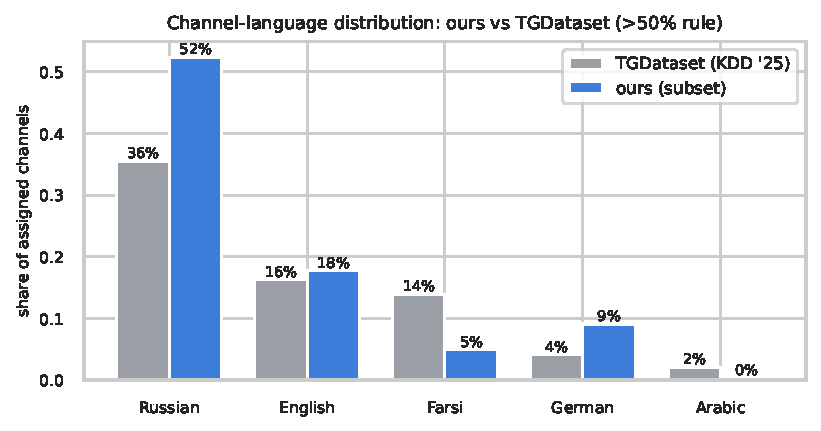
\includegraphics[width=\textwidth]{figures/res_language_distribution}
\caption[Channel language distribution.]{Majority-language distribution across channels with a detected dominant language. Russian dominates, followed by English, German, Ukrainian, and Farsi.}
\label{fig:res-language}
\end{figure}

\begin{figure}[htbp]
\centering
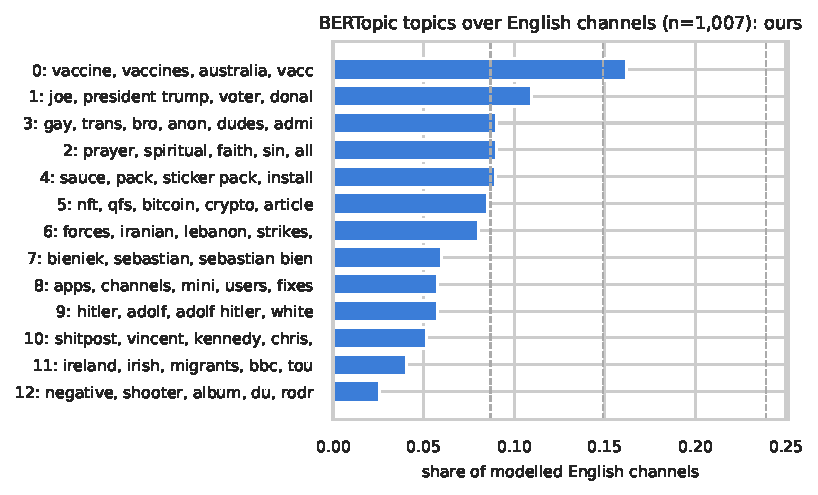
\includegraphics[width=\textwidth]{figures/res_topic_shares}
\caption[Topic shares.]{Channel topic shares from a BERTopic model~\cite{grootendorst2022} over English-language channel content.}
\label{fig:res-topics}
\end{figure}

\begin{figure}[htbp]
\centering
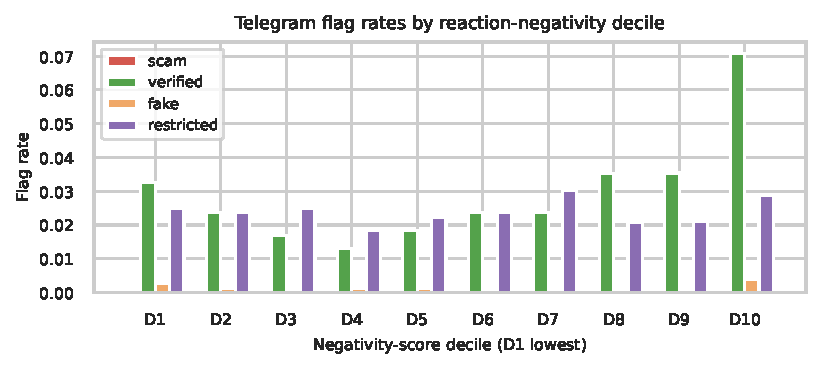
\includegraphics[width=\textwidth]{figures/res_reaction_negativity_flag_rates}
\caption[Verified rate across reaction-negativity deciles.]{Channel flag rates across deciles of audience reaction negativity. The verified rate roughly doubles from the most-positive to the most-negative decile: verification tracks prominence and controversy, not vetted safety.}
\label{fig:res-verified}
\end{figure}

\begin{figure}[htbp]
\centering
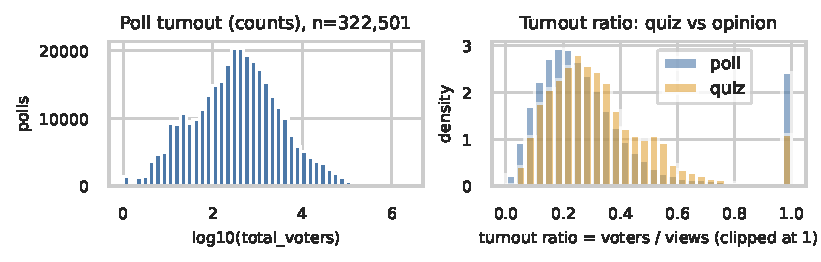
\includegraphics[width=\textwidth]{figures/res_poll_turnout}
\caption[Poll turnout.]{Poll turnout across the corpus. A subset of polls carries per-option vote tallies, making vote-distribution shape analysable.}
\label{fig:res-polls}
\end{figure}

\begin{figure}[htbp]
\centering
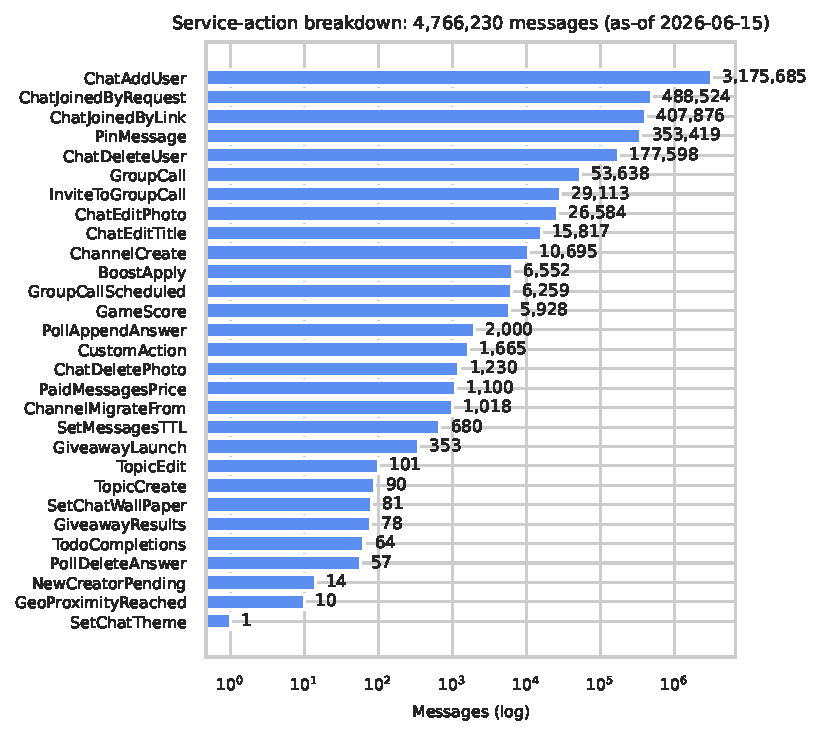
\includegraphics[width=\textwidth]{figures/res_service_actions}
\caption[Service actions.]{Distribution of service actions (pinning, migrations, membership and monetisation events) captured as structured records.}
\label{fig:res-service}
\end{figure}

\subsection{What We Did Not Find, and What to Distrust}
\label{sec:res-nulls}

Two results are valuable precisely as negatives. First, there is no large-scale automated sockpuppet network detectable from profile pictures: across the $12{,}065$ channels scraped for messages, profile images are almost all distinct ($10{,}805$ distinct images), and we find no notable near-duplicate clusters. Second, longitudinal metadata change is tiny: over consecutive-snapshot pairs, only the profile picture ($1.6\%$) and description ($1.2\%$) change appreciably, while the title ($0.3\%$), username ($0.1\%$), and the boolean flags are near zero (Table~\ref{tab:res-metadata}). This is partly a real null and partly a snapshot-density limitation; its concrete value is that it corrected an earlier inflated rate caused by privacy-blanking double-counting.

A final caveat concerns one trust flag that downstream users should treat with caution: \texttt{is\_scam} is set on only five channels and never changes across the snapshot history, so any analysis of scam status over time should rely on \texttt{is\_fake}, \texttt{is\_restricted}, or verification status instead.

\begin{table}[htbp]
\centering
\caption[Consecutive-snapshot metadata change rates.]{Per-pair change rates for channel metadata fields over consecutive snapshots. Only the profile picture and description change appreciably; \texttt{is\_scam} never flips.}
\label{tab:res-metadata}
\small
\setlength{\tabcolsep}{6pt}
\begin{tabular}{@{}lrr@{}}
\toprule
\textbf{Field} & \textbf{Changes / pairs} & \textbf{Rate} \\
\midrule
Profile picture (\texttt{photo\_hash}) & $346 / 21{,}594$ & $1.60\%$ \\
Description                            & $266 / 23{,}116$ & $1.15\%$ \\
Title                                  & $65 / 23{,}116$  & $0.28\%$ \\
Username                               & $14 / 20{,}051$  & $0.07\%$ \\
\texttt{is\_restricted}               & $16 / 23{,}191$  & $0.07\%$ \\
\texttt{is\_scam}                     & $0 / 23{,}191$   & $0.00\%$ \\
\bottomrule
\end{tabular}
\end{table}

%======================================================================
\section{Showcase: USA/Israel--Iran War}
\label{sec:res-war}
%======================================================================

The preceding sections each exercised one capability layer in isolation. A single current event exercises several at once, and the 2026 USA/Israel--Iran war (opening strike $28$~February~2026) is the showcase. The analysis draws on two curated companion databases held alongside the main corpus, \texttt{tgdataset\_iran} and \texttt{tgdataset\_israel}, each built mainly from official and semi-official sources. Each is a bounded crawl: it scrapes a set of official seed channels, their linked comment groups, and the channels they forward from at one hop, and goes no further. The official cohort the figures below rest on is the scraped seeds, $20$ of $27$ on the Iranian side and $25$ of $42$ on the Israeli; counting the comment groups and first-degree forwards as well, the two crawls cover $493$ and $416$ scraped channels respectively (Iran $20$ seeds, $95$ comment groups, $378$ forwards; Israel $25$, $123$, $268$). On the Iranian side these are state news agencies (IRNA, Fars, Mehr, ISNA) together with government and IRGC-affiliated outlets (Press~TV, Tehran~Times, the Khamenei channel); on the Israeli side the IDF, the Home Front Command, the police, government ministries, the emergency services MDA and United~Hatzalah, and the major national outlets. Two commitments run through everything below. Every result is a shift measured against each side's own pre-war baseline (November~2025 to February~2026).

\paragraph{Why Iran is a useful case.}
Section~\ref{sec:res-content} flagged the Farsi cohort as notably ban-resilient: Telegram has remained a usable Iranian information channel through the state's 2018 attempt to block it, with $99\%$ of channels active before the ban still active afterward and most still active in 2026. The wartime data bears this out from the other direction, the Farsi cohort staying near $0\%$ restricted across every restriction reason while the fighting was hottest (Section~\ref{sec:res-restriction}). A surface the state cannot easily suppress is exactly where an official wire is worth watching, which is why the Iranian side anchors the comparison.

\paragraph{The ``flat Iran'' artefact, corrected.}
The snowball reading of the Iranian side, taken from language cohorts in the main corpus, looked flat: pooled daily Farsi volume rose only $1.17\times$ over its pre-war level, the median Farsi channel posted about $0.1\times$ (a net decline), and roughly $30\%$ of channels went silent. Read like for like against the curated Israeli cohort, that picture reverses. The official Iranian wire surged $2.05\times$ over its own pre-war baseline, and the surge is broad-based: the median official Iranian channel more than doubled its output ($2.23\times$), none went silent, and $95\%$ posted more. The Israeli official surface lifts comparably ($2.94\times$ pooled, median $1.78\times$, none silent, $90.9\%$ up). The methodological point is the headline. Snowball sampling, by mixing mostly-dormant grassroots channels into the Farsi cohort, masked a real and broad official mobilisation that only a like-for-like curated comparison recovers (Figures~\ref{fig:res-war-volume} and~\ref{fig:res-war-concentration}).

\begin{figure}[htbp]
\centering
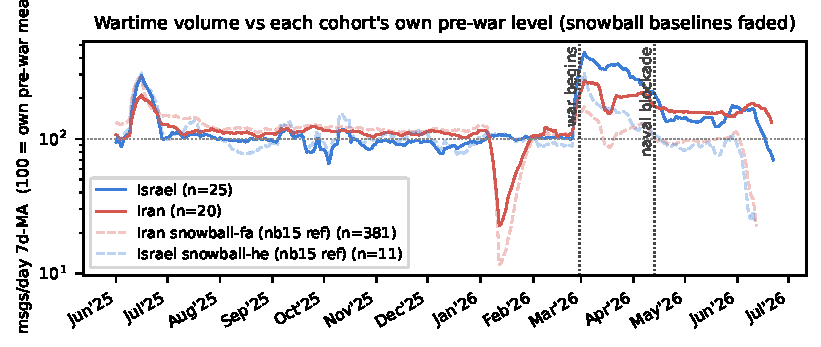
\includegraphics[width=\textwidth]{figures/res_official_volume_index}
\caption[Two official wartime surfaces.]{Daily message volume for the two official cohorts, each indexed to $100$ at its own pre-war (November~2025 to February~2026) mean, with the snowball Farsi and Hebrew language cohorts overlaid faded as the earlier baselines. Both official wires surge over their own pre-war level (Israel $2.94\times$, Iran $2.05\times$); the snowball Farsi line ($1.17\times$) is the flat reading the curated comparison reverses.}
\label{fig:res-war-volume}
\end{figure}

\begin{figure}[htbp]
\centering
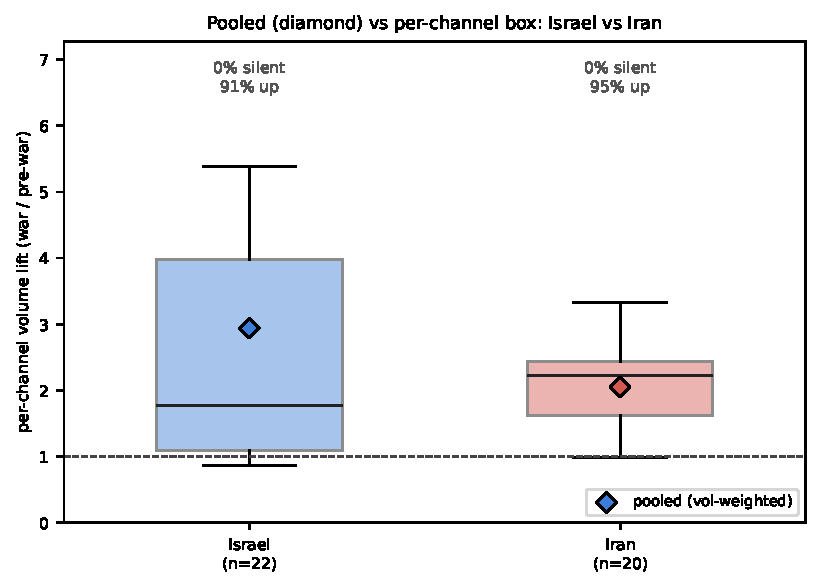
\includegraphics[width=\textwidth]{figures/res_per_channel_lift}
\caption[Pooled versus typical official channel.]{Per-channel war-versus-pre volume lift for each official cohort: pooled lift (diamond) against the channel-level distribution (box). On both cohorts the median channel more than doubled (Iran $2.23\times$, Israel $1.78\times$) with none falling silent, the opposite of the snowball Farsi cohort's median $\sim0.1\times$ and $\sim30\%$ silent. The broad official mobilisation is not a loud-minority effect.}
\label{fig:res-war-concentration}
\end{figure}

\paragraph{Where the surge comes from.}
Splitting each cohort's volume into an extensive margin (how many channels are active) and an intensive margin (how much each active channel posts) locates the surge. Neither official cohort loses channels at the opening strike: the active-channel step is $1.17\times$ for Israel and $0.99\times$ for Iran. Both instead ramp on the intensive margin (Israel $3.76\times$, Iran $2.45\times$), the same channels simply posting far more. This is the opposite of the snowball Farsi cohort, whose active-channel count roughly halved at the opening strike ($0.56\times$): the apparent collapse in the snowball reading was its dormant grassroots tail going quiet, not the official wire contracting.

\paragraph{Institution-fixed multilingual escalation.}
The cleanest, selection-free signal holds a single institution fixed and compares its parallel language arms, so any divergence is audience targeting rather than which channels were sampled. The pattern is symmetric across both states: each escalates its English or international arm hardest. The IDF lifts its English arm $5.39\times$ against $3.87\times$ Hebrew and $2.82\times$ Arabic; IRNA lifts English $1.64\times$ against $1.14\times$ Persian; Mehr lifts English $2.46\times$ against $1.90\times$ Persian; and the English-only Tehran~Times rises $47.5\times$ from a near-dormant pre-war base, a figure to read as a direction (an international arm switched on for the war) rather than a precise multiplier. With the institution held fixed, there is no sampling confound left, and the wartime priority on both sides is plainly the international narrative (Figure~\ref{fig:res-war-arms}).

\begin{figure}[htbp]
\centering
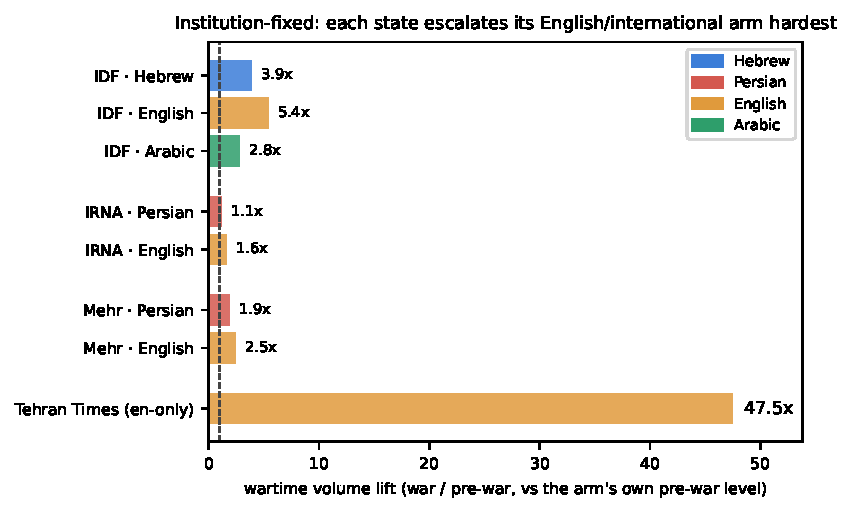
\includegraphics[width=\textwidth]{figures/res_institution_arms}
\caption[English arm escalates hardest, both states.]{War-versus-pre volume lift for the parallel language arms of single institutions (IDF he/en/ar, IRNA and Mehr fa/en, Tehran~Times en-only), each arm indexed to its own pre-war mean. Because the institution is fixed, the divergence is audience targeting, not channel selection: each state escalates its English or international arm hardest.}
\label{fig:res-war-arms}
\end{figure}

\paragraph{Editorial tempo and the air-war clock.}
The war also pushed both wires off their peacetime editorial clock. The share of posting in the local overnight window roughly tripled on each side (Israel $4.0$ to $13.4\%$, Iran $4.5$ to $15.5\%$), as office-hours posting gave way to a more around-the-clock reactive cadence. An exogenous timing signal corroborates the shift: the Israeli Home Front Command's public missile-alert feed, which fired $14{,}122$ alerts over the war window, correlates at $r\approx0.61$ with the daily output of the official Iranian wire (Figure~\ref{fig:res-war-clock}). The two surfaces are keyed to the same air-war clock.

\begin{figure}[htbp]
\centering
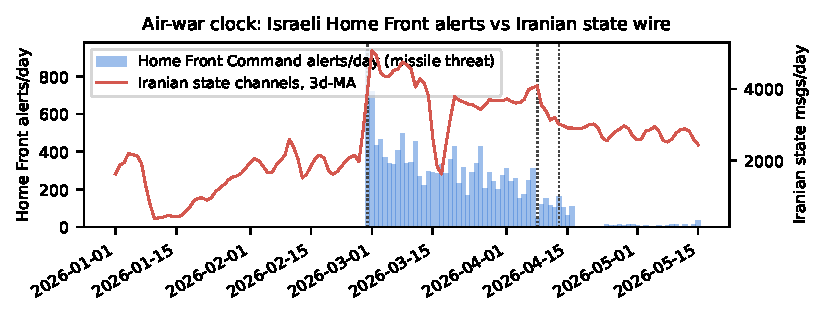
\includegraphics[width=\textwidth]{figures/res_homefront_clock}
\caption[Home Front alerts against the Iranian state wire.]{Daily Israeli Home Front Command missile alerts ($14{,}122$ over the war window) against the daily output of the Iranian state wire. The two track the same exogenous air-war clock ($r\approx0.61$), an external timing reference that neither side controls.}
\label{fig:res-war-clock}
\end{figure}

\paragraph{Audience reaction valence.}
Audience reaction valence, a language-neutral positive-minus-negative score over the structured reaction surface, swung far more on the Iranian side. The Iranian official audience moved from $+0.103$ to $+0.662$ (a shift of $+0.56$ over roughly $2.9$~million wartime reactions), against the Israeli audience's $+0.229$ to $+0.318$ ($+0.09$ over about $0.44$~million). Read as an audience-approval proxy and compared as each side's own shift rather than across sides, the Iranian state audience rallied around its wire far harder than the Israeli audience did around its own.

\paragraph{Narrative convergence and overlap.}
Whether the two surfaces are even covering the same war can be measured directly with cross-lingual sentence embeddings (\texttt{paraphrase-multilingual-MiniLM-L12-v2})~\cite{reimers2019,reimers2020} over each side's domestic-language broadcasts. Daily cross-side centroid cosine similarity is high throughout and peaks at $0.914$ on the $8$~April ceasefire (mean $0.851$ over the $61$-day window): both wires orient to the same exogenous events (Figure~\ref{fig:res-war-framing}). The overlap is asymmetric, though. At a cosine threshold of $0.6$, $95.9\%$ of Iranian broadcasts have an Israeli semantic counterpart, against only $79.3\%$ the other way: the Israeli wire carries more siloed home-front, municipal, and health content with no Iranian analogue, while the Iranian wire maps almost entirely onto the shared war narrative.

\begin{figure}[htbp]
\centering
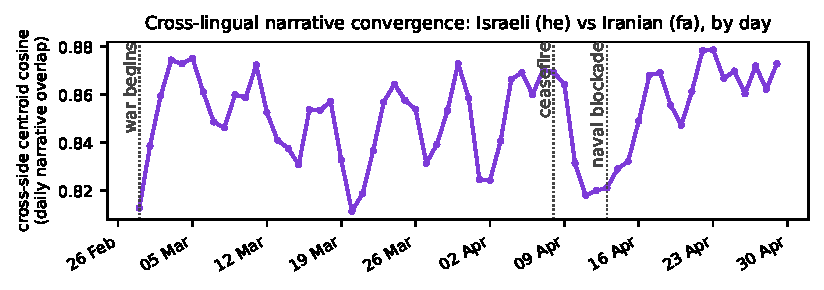
\includegraphics[width=\textwidth]{figures/res_framing_convergence}
\caption[Cross-side narrative convergence.]{Daily cross-side centroid cosine similarity between the two official wires' domestic-language broadcasts, from cross-lingual sentence embeddings. Convergence is high throughout and peaks at $0.914$ on the $8$~April ceasefire (mean $0.851$ over $61$ days): both surfaces orient to the same events. The cosines are approximate; read the temporal shape, not absolute levels.}
\label{fig:res-war-framing}
\end{figure}

\paragraph{Audience toxicity.}
The comment audiences under the two wires also differ in hostility. Scored with the \texttt{textdetox} XLM-R toxicity classifier~\cite{dementieva2024}, the Iranian official comment audience runs $23.4\%$ toxic against the Israeli audience's $18.6\%$. The English-language sections are the nastiest on both sides (around $30\%$ each), and on the Arabic axis, the firmest cross-lingual comparison for this classifier, the Iranian audience ($16.4\%$) again tops the Israeli ($10.8\%$) (Figure~\ref{fig:res-war-toxicity}). These are classifier labels on bounded per-side samples (about $9{,}000$ comments each), so the contrast and its direction carry the reading, not the exact percentages.

\begin{figure}[htbp]
\centering
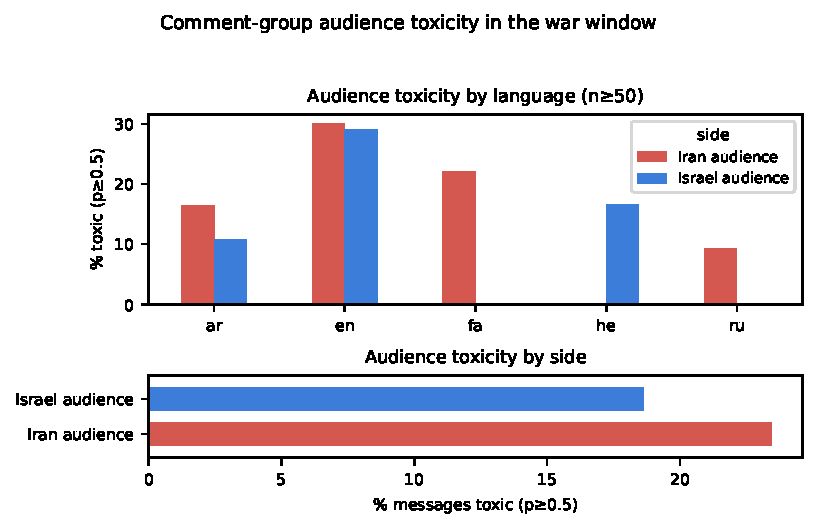
\includegraphics[width=\textwidth]{figures/res_toxicity_by_side}
\caption[Two official audiences' toxicity.]{Toxic-comment share in the two official cohorts' discussion-group audiences, scored with the \texttt{textdetox} XLM-R classifier. Top: by audience language; bottom: by side. The Iranian audience ($23.4\%$) runs more toxic than the Israeli ($18.6\%$); on the Arabic axis (the firmest cross-lingual comparison) the same direction holds ($16.4\%$ against $10.8\%$). Bounded samples of about $9{,}000$ comments per side; read the contrast, not the point values.}
\label{fig:res-war-toxicity}
\end{figure}

\paragraph{Polls and audience composition.}
Two smaller layers round out the showcase. Polls behave as state opinion probes: the official Iranian wire runs them more frequently and to several times the reach of the Israeli wire (median $4{,}310$ voters against $738$), though poll frequency fell on both sides during the war as hard news displaced engagement-polling. And the comment audiences differ in composition: the Iranian official audience is markedly more multilingual (Farsi $52\%$, English $24\%$, Arabic $14\%$) than the Israeli (Hebrew $66\%$, English $25\%$, Arabic $5\%$), consistent with the international-arm escalation seen on the broadcast side.

\paragraph{What the showcase exercises.}
A single event therefore exercises the comment, reaction, poll, language, and (corpus-wide) deletion layers at once, and the analysis is method-led throughout: per-cohort indexing against each side's own baseline, a pooled-versus-median decomposition that overturns the general snowball reading, institution-fixed multilingual contrasts, and an exogenous timing clock. Every figure here is a lead about how two state information surfaces behaved, read against each side's own baseline on small, separately-sampled cohorts in a companion database. The Iranian official cohort in particular is a lower bound: $20$ of $27$ official seeds were captured across the two scrape runs, and the seven missing include heavyweights such as Tasnim and Sepah/IRGC, so its volume and concentration figures understate the full official wire.

\chapter{Conclusions}
\label{chap:conclusion}

This thesis set out from a structural gap in the public Telegram record: existing corpora, however large, are snapshots that record each channel once and discard almost everything that makes a channel a living object over time, its edits, its deletions, and the drift of its metadata. The resolution is a scraper that revisits public channels on a schedule, recurses into their linked discussion groups, and on each visit detects edits and deletions and snapshots channel metadata, all within Telegram's rate limits. The corpus it produces, TGDataset2, is the first general-purpose Telegram dataset to carry message edits with their before-and-after text, deletions, and longitudinal metadata, alongside a structured engagement-and-comment surface. That capability is bought with a deliberate trade of breadth for depth: $12{,}065$ channels each revisited over time.

Across the new layers, a widely used raw signal repeatedly overstates the phenomenon it is taken to measure, while longitudinal or structured capture supplies the corrected picture. The \texttt{edit\_date} timestamp over-counts human editing by roughly an order of magnitude, because $93\%$ of the edits caught in full leave the message text byte-identical, and only the before/after archive separates genuine rewrites from media and markup churn. The raw forward flag overstates editorial reposting by about a third, because a third of flagged forwards are auto-mirror copies of a channel's own posts into its discussion group; removing them moves the forward ratio from $18.3\%$ to $12.1\%$. The reply-pointer count overstates comments-on-posts by roughly $42\%$, because not every reply anchors on a broadcast post, and anchoring-aware accounting is what separates a true comment section from in-group chat.

%======================================================================
\section{Limitations}
\label{sec:limitations}

This section consolidates the known limitations of the dataset and the system that produced it. Each item is cross-referenced to the methodology section where the corresponding design decision and its rationale are discussed, so a reader can trace every limitation back to the trade-off that produced it.

\paragraph{Sampling bias from forward-only discovery.}
Channel discovery relies exclusively on forwarded-message references; username resolution is disabled to preserve the rate-limit budget for message collection (Section~\ref{sec:channel-discovery}). Channels that are only reachable through \texttt{@}-mentions or \texttt{t.me/} links, without ever being forwarded, are therefore under-sampled. More broadly, snowball sampling, the chain-referral technique that expands a seed set by following inter-channel references, is known to over-represent high-degree nodes and under-cover weakly connected regions of the network~\cite{wagner2017}. This bias is not merely theoretical here: as Section~\ref{sec:res-frontier} shows, the unreachable frontier is organised rather than random (it clusters by theme and includes the linked discussion groups of major channels), and roughly $14.5\%$ of cited \texttt{t.me} links are invite-only or web-preview references that the scraper structurally cannot resolve, a hard ceiling rather than a backlog. Any finding derived from the dataset should be interpreted in light of these biases.

\paragraph{Count-based deletion heuristic.}
The combined pass decides whether to perform a full-history deletion scan by comparing the server-reported message count against the locally stored count (Section~\ref{sec:combined-pass}). If the number of deletions between two visits is exactly offset by an equal number of new messages, the counts balance and the deletion is silently missed until a subsequent visit restores the imbalance. The full alternative, a history pull on every visit, was rejected as infeasible within Telegram's rate limits. A consequence specific to the analysis is that the deletion layer is also a detection-time record: a deleted row's timestamp marks when the scraper noticed the deletion on revisit, not when it happened, and the deletion-detection window is short (it begins in May~2026), so all deletion findings characterise the collected deleted set rather than Telegram's deletion semantics in general.

\paragraph{Edit-detection blind spot beyond the overlap window.}
On clean runs the combined pass takes Path~B (Section~\ref{sec:combined-pass}), which only re-fetches the last $N$ messages below \texttt{highest\_id} (default $N=100$) to check for edits. Edits to messages older than $N$ are therefore invisible until the same channel happens to enter Path~A for an unrelated reason: a detected deletion or a crash-triggered forced recheck (Section~\ref{sec:robustness}). These three mechanisms guarantee that no edit remains hidden indefinitely, but the latency until discovery is not bounded by $N$ alone. As a result the before/after edit archive is a selected slice, weighted toward old posts caught changing on re-scrape, and \texttt{edit\_date} remains only an upper bound on human editing (Section~\ref{sec:res-edits}). Increasing $N$ widens the window at linear API-call cost per channel per run.

\paragraph{Posted-and-deleted between visits.}
A message that is both posted and deleted in the interval between two of our visits is invisible by construction: we never observed it, the database has no row to flag, and \texttt{server\_total} does not reflect it either. This is an unavoidable property of any polling scraper and is independent of the detection strategy.

\paragraph{Race between the count ping and the new-message pull.}
The cheap path (Section~\ref{sec:combined-pass}) reads \texttt{server\_total} first and then fetches new messages. A post that lands in the few seconds between those two operations is counted in $n_{\mathrm{new}}$ but not in \texttt{server\_total}, inflating $n_{\mathrm{expected}}$ and producing a false-positive deletion signal; symmetrically, a deletion in the same window can produce a confusing comparison. The consequence is at worst one redundant Path~A run, never data loss or corruption: the full pull finds no missing IDs and the next run sees consistent counts. The races are rare enough that no mitigation is implemented. Alignment runs (Section~\ref{sec:alignment}) widen this race from the gap between two API calls to the gap between the alignment trigger and each channel's turn (minutes to hours), and change its direction: because \texttt{server\_total} remains live-global while $n_{\mathrm{new}}$ is bounded by the cutoff $t_c$, post-cutoff activity can \emph{mask} deletions rather than produce false positives. The consequence is still bounded: the regular scrape that follows every alignment run sees no cutoff, runs an exact cheap check, and catches any deletions that were masked during alignment.

\paragraph{Temporal drift across channels.}
Because channels are scraped sequentially by a single process, the per-channel metadata snapshots within a single run are captured at different wall-clock moments. The alignment snapshot protocol (Section~\ref{sec:alignment}) guarantees that every channel's \emph{message} stream is captured up to the same cutoff $t_c$, but the \emph{metadata} snapshots remain spread across the alignment cycle. Drift is therefore bounded by the alignment interval ($30$ days by default) rather than eliminated. The practical effect is visible in the analysis: the consecutive-snapshot change rates of Section~\ref{sec:res-nulls} are constrained as much by snapshot density as by genuine stability.

\paragraph{Bounded crash-window data loss.}
Messages are committed to the database per batch rather than per message (Section~\ref{sec:robustness}). A crash at the worst possible moment can therefore lose the in-flight batch (up to $100$ messages per affected channel). The lost messages are re-fetched on the next run because they sit above the stored \texttt{highest\_id}, so the loss is bounded and self-healing rather than permanent.

\paragraph{Dormant trust flag.}
The \texttt{is\_scam} flag should not be used as-is by downstream reusers (Section~\ref{sec:res-nulls}): it is effectively dead (five channels, never flipped), so any moderation-over-time analysis should rely on \texttt{is\_fake}, \texttt{is\_restricted}, or verification.

\paragraph{Companion database is separate and shallow.}
The official-Israel arm of the war showcase (Section~\ref{sec:res-war}) lives in a separate companion database, seeded from official Israeli channels and expanded by a single snowball pass, rather than in the main corpus. Cross-side comparisons are therefore reconciled in analysis on small cohorts, and they are cross-sampling-method (official-seeded voices against a subset of TGDataset's channels) as well as cross-database, so they are read as institution-fixed contrasts and per-channel shapes rather than as absolute cross-side volumes. The companion database is also shallow in time, with little edit or deletion depth, so the Israeli arm uses volume, cadence, and reactions only.

\paragraph{Scope boundaries.}
Three deliberate scope boundaries further narrow what the dataset captures. Media files attached to messages are not downloaded (Section~\ref{sec:schema}); only the media-type indicator is preserved. The scraper is designed to run as a single process on a single machine; multi-instance or distributed scraping is out of scope (Section~\ref{sec:robustness}). The unit of analysis is public channels only; private chats, groups, and user-level messages are not collected.

\paragraph{Measurement validity of derived labels.}
The analytical layers lean on off-the-shelf models applied largely cross-lingually, without task-specific ground-truth validation on this corpus: the \texttt{textdetox} XLM-R toxicity classifier~\cite{dementieva2024}, Claude Sonnet~4.6 edit labelling~\cite{claudesonnet2026}, a multilingual named-entity tagger~\cite{tedeschi2021}, BERTopic~\cite{grootendorst2022}, language detection, and cross-lingual sentence embeddings~\cite{reimers2020}, together with reaction valence and turnout read as audience-sentiment proxies. The caveat is that such results carry direction and contrast rather than calibrated absolute levels, and the firmest cross-side comparison holds the language fixed, as the war section does when it reads audience toxicity off both sides' shared Arabic sections rather than across Farsi and Hebrew.

\paragraph{Corpus composition and generalisability.}
Beyond the forward-only discovery bias above, the corpus is seeded from TGDataset's channels (Section~\ref{sec:deployment}) and is Russophone-heavy (Russian is $52\%$ of majority-language channels), so it is a particular slice of Telegram rather than a representative sample. Every rate reported in this thesis, deletion, forward, restriction, and edit, is therefore a within-corpus rate, not a platform-wide prevalence estimate, and should be read as such.

%======================================================================
\section{Future Work}

The system and corpus open more avenues than this thesis closes. The richest of them are analyses the new layers now make directly possible.

\begin{itemize}
  \item \textbf{Longitudinal moderation at scale.} The deletion-detection window only opened in May~2026, so the $2.42$\,M detected deletions are a detection-time sample rather than a record of moderation dynamics. Sustained running turns that sample into genuine deletion \emph{dynamics}, who deletes, when, and how removals propagate, and lets restriction flags and metadata be read as time series. This is the direct route from the near-null longitudinal-metadata result and the partial deletion sample of this thesis to measurable trajectories.
  \item \textbf{Edits as a research signal.} The before/after archive (currently $36{,}016$ edits caught in full) is the diffable layer no other general-purpose corpus holds. Scaled up, it supports the study of misinformation correction, stealth edits, and coordinated narrative changes from the text of the change itself rather than from a bare timestamp.
  \item \textbf{The comment layer as a social object.} With $333.2$\,M discussion messages, the comment side can carry commenter-network, returning-audience, and thread-structure studies. The anchoring-aware accounting of Section~\ref{sec:res-layers} is what makes them tractable, separating genuine comment sections from in-group chat before any measurement begins.
\end{itemize}

A smaller set of system extensions would unlock and sharpen those analyses. Lower-latency edit and deletion detection (an adaptive overlap window, selective history pulls, and a limited real-time API path in the spirit of Kireev et al.~\cite{propaganda2025}) would catch messages posted and deleted between visits and recover true deletion timestamps rather than detection times; denser, event-triggered metadata snapshots would resolve the temporal-drift limitation that holds the current metadata result near null; re-enabled username and link discovery under a separate rate budget would shrink the organised frontier; optional media or perceptual-hash capture would let the sockpuppet null result be revisited on image content rather than profile pictures alone.

%======================================================================

Making content \emph{dynamics} observable, not just content, is the shift the title names, and it is what changes the questions one can put to Telegram: from what a channel said once to how its public record was edited, deleted, and otherwise managed over time. That the system does this openly and reproducibly from the documented defaults of Table~\ref{tab:config} is the point. It lowers the barrier for others to ask those questions of the platform too.


\appendix
\chapter{Edit-labelling prompt}
\label{app:edit-prompt}

This appendix reproduces the prompt used to label the $2{,}356$ text-changing edits discussed in Section~\ref{sec:res-edits}. Pairs are labelled in batches of $25$, one model call per batch. For each call the prompt below is filled in by listing the batch's pairs under \texttt{Items:}, one JSON object per pair carrying its \texttt{id}, archived \texttt{before} text, and current \texttt{after} text; the model then returns a JSON array with one label object per pair. The labels are the fixed taxonomy shown; the substantive/non-substantive split reported in the text is then derived from the label, with \texttt{cosmetic} and \texttt{mechanical\_counter} counted as non-substantive and the rest as substantive.

\begin{lstlisting}[numbers=none,caption={Edit-type labelling prompt, as sent to Claude Sonnet~4.6.},captionpos=b,label={lst:edit-prompt}]
You are annotating EDITS to Telegram posts. For each item you get the BEFORE text (the archived prior version) and the AFTER text (the current version). Assign exactly ONE primary label = the *dominant* kind of change between BEFORE and AFTER. The corpus is multilingual (Russian-heavy, plus Farsi, German, Hebrew, etc.) - judge the change, not the language.

Labels (choose one):
- cosmetic: spelling/typo, spacing, punctuation, emoji, markup, or hashtag only; meaning unchanged.
- mechanical_counter: only an auto-updating tally changed (poll votes, reaction/comment/view counts); not an editorial edit.
- factual_correction: a number, date, name, place, or fact changed to correct or update it (meaning changes).
- addition: new substantive content, links, promo/CTA, or a status note appended or inserted.
- removal: substantive content cut or retracted, or the post emptied.
- tone_rewrite: wording rephrased (soften/harden/restyle) without adding or removing facts.
- compliance_annotation: a state- or platform-mandated label/disclaimer added or removed (e.g. 'foreign agent', ToS notice).
- multi: two or more co-equal substantive change types in one edit.
- other: none of the above.

Also return `note`: <=12 words naming the concrete change.

Output ONLY a JSON array, one object per item, no prose and no markdown fences:
[{"id": "<id>", "label": "<label>", "note": "<...>"}]

Items:
{"id": "<channel_id>:<message_id>", "before": "<archived text>", "after": "<current text>"}
...
\end{lstlisting}


\backmatter

\bibliographystyle{sapthesis}
\bibliography{bibliography/references}

\end{document}
